\documentclass[letterpaper, onecolumn, 11pt]{report}
\usepackage[utf8]{inputenc}
%\usepackage[spanish]{babel}
\usepackage{amsmath}
\usepackage{amssymb}
\usepackage{siunitx}
\usepackage{graphicx}
%\usepackage{txfonts} %bkn
\usepackage{physics}
\usepackage{wrapfig}
\usepackage{hyperref}
\usepackage{marginnote}
\usepackage{caption}
\usepackage{amsfonts}
%\usepackage{draculatheme} %Agregar draculatheme.sty  al directorio del proyecto LaTeX
%\spanishdecimal{.}
\usepackage{hyperref}
\usepackage{marginnote}
\hypersetup{colorlinks=true, linkcolor=red}

\newtheorem{teo}{Theorem}
\newtheorem{axiom}{Axiom}
\newtheorem{example}{Example}
\newtheorem{sol}{Solution}



\renewcommand*{\marginnotevadjust}{-0.1cm}
\renewcommand*{\marginfont}{\footnotesize}
\usepackage[right=4.5cm,left=2cm,top=3cm,bottom=3.0cm]{geometry}
\begin{document}
\sffamily
\begin{center}

\

\vspace{6.5cm}

\rule{15cm}{0.1cm}

\vspace{1.5cm}

{\huge \textsc{\textbf{Quantum Mechanics}}}

\vspace{1.5cm}

\rule{15cm}{0.1cm}

\vspace{1.5cm}
Diez B. Borja


\today

\newpage
\setcounter{page}{1}
\pagenumbering{roman}

\pagestyle{plain}
\chapter*{Preface}
\addcontentsline{toc}{chapter}{Preface}
\bigskip
\bigskip
\bigskip
\bigskip
\bigskip
\bigskip


\emph{This notes has been written by \href{https://github.com/10BlackHole}{B. Diez} mainly from Introduction to Quantum Mechanics by David J. Griffiths and own knowledge.}

\end{center}
%\title{\Huge\textbf{{Quantum Mechanics}}}
%\author{Diez B. Borja}
%\maketitle
\tableofcontents
\pagenumbering{arabic}
\setcounter{page}{1}
%\input{cap/the-wave-function.tex}
%\chapter{Time-Independent Schrodinger Equation}
\section{Stationary States}
Wa talked a lot about the wave function, and how you use it to calculare various quantities of interest. But, how do get $\Psi(x,t)$ in the first place? We need to solce the Schrodinger equation,
\begin{equation}\label{2.1}
	i\hbar\pdv{\Psi}{t}=-\frac{\hbar^2}{2m}\pdv[2]{\Psi}{x}+V\Psi
\end{equation}
for a specified potential\footnote{It is tiresome to keep saying "potential energy function", so most people jus call $V$ the "potential", even though this invites occasional confusion with electric potencial, which is actually potential energy per unit charge.} $V(x,t)$. In this chapter (and most of this book) I shall assume that $V$ is \textit{independent} of $t$. In that case the Schrodinger equation can be solved by the method of \textbf{separation of variables}: We look for solutions that are simple \textit{products},
\begin{equation}\label{2.2}
	\Psi(x,t)=\psi(x)\varphi(t)
\end{equation}
where $\psi$ is a function of $x$ alone, and $\varphi$ is a function of $t$ alone. 

For separable solutions we have
\begin{equation*}
	\pdv{\Psi}{t}=\psi\dv{\varphi}{t},\qquad \pdv[2]{\Psi}{x}=\dv[2]{\psi}{x}\varphi
\end{equation*}
(\textit{ordinaty} derivatives, now), and Schrodinger equation reads
\begin{equation}
	i\hbar\dv{\varphi}{t}=-\frac{\hbar^2}{2m}\dv[2]{\psi}{x}\varphi + V\psi\varphi
\end{equation}
Or, dividing through by $\psi\varphi$:
\begin{equation}\label{2.3}
	i\hbar\frac{1}{\varphi}\dv{\varphi}{t}=-\frac{\hbar^2}{2m}\frac{1}{\psi}\dv[2]{\psi}{x}+V
\end{equation}

Now, the left side is a function of $t$ alone, and the right side is a function of $x$ alone\footnote{Note that this would not be true if $V$ were a function of $t$ as well as $x$.}. The only way this can possibly be true is if both sides are in fact \textit{constant} -- otherwise, by varying $t$, I could change the left side without touching the right side, and the two would no lonegr equal. For reasons that will appear in a moment, we shall call the separation constan $E$. Then
\begin{equation*}
	i\hbar\frac{1}{\varphi}\dv{\varphi}{t}=E
\end{equation*}
or
\begin{equation*}\label{2.4}
	\dv{\varphi}{t}=-\frac{iE}{\hbar}\varphi
\end{equation*}
and
\begin{equation}
	-\frac{\hbar^2}{2m}\frac{1}{\psi}\dv[2]{\psi}{x}+V=E
\end{equation}
or
\begin{equation}\label{2.5}\marginnote{Time-independent Schrodinger equation}
	\boxed{-\frac{\hbar^2}{2m}\dv[2]{\psi}{x}+V\psi=E\psi}
\end{equation}
Separation of variables hs turned a \textit{partial} differential equation into \textit{two ordinary} differential equations (\ref{2.4}) and (\ref{2.5}). The first, (\ref{2.4}) is easy to solve (just multiply through by $\dd t$ and integrate); the general solution is $C\exp(-iEt/\hbar)$, but we might as well absorb the constant $C$ into $\psi$ (since the quantity of interest is the product $\psi\varphi$). Then
\begin{equation}\label{2.6}
	\varphi(t)=e^{-iEt/\hbar}
\end{equation}
The second equation (\ref{2.5}) is called the \textit{time-independent Schrodinger equation} we can go further with it until the potencial $V(x)$ is specified.

The rest of thus chapter will be devoted to solving the time-independent Schrodinger equation, fot a variety of simple potentials. But before I get to that you have every right ask: What's so great about separable solutions? After all, most solutions so the (time dependent) Schrodinger equation do not take the form $\psi(x)\varphi(t)$. I offer three answers--two of them physical, and one mathematical:
\begin{enumerate}
	\item They are \textbf{stationaty states}. Although the wave function itself,
\begin{equation}\label{2.7}
	\Psi(x,t)=\psi(x)e^{-iEt/\hbar}
\end{equation}
does (obviously) depende on $t$, the \textit{probability density},
\begin{equation}\label{2.8}
	|\Psi(x,t)|^2=\Psi^*\Psi=\psi^*e^{+iEt/\hbar}\psi e^{-iEt/\hbar}=|\psi(x)|^2
\end{equation}
does not--the time-dependence cancels out\footnote{For normalizable solutions, $E$ must be real}. The same thing happens in calculate the expectation value of any dynamil variable; (\ref{1.36}) reduces to
\begin{equation}\label{2.9}
	<Q(x,p)>=\int\psi^*Q\left(x,\frac{\hbar}{i}\frac{\dd}{\dd x}\right)\psi\dd x
\end{equation}
\textit{Every expectation value is constant in time}; we might as well drop the factor $\varphi(t)$ altogether, and simply use $\psi$ in place of $\Psi$. In particular, $<x>$ is constant, and hence $<p>=0$ (See (\ref{1.33})). Nothing ever happens in a stationary state.

\item They are states of \textit{definite total energy}. In classical mechanics, the total energy (kinetic plus pontential) is called the \textbf{Hamiltonian}:
	\begin{equation}\label{2.10}
	H(x,p)=\frac{p^2}{2m}+V(x)
\end{equation}
The corresponding Hamiltonian \textit{operator}, obtained by the canonical substitution $p\to (\hbar/i)(\partial /\partial x)$, is therefore\footnote{Whenever confusion might arise. I'll put a "hat" on the operator, to distinguish it from the dynamical variable it represents.}
\begin{equation}\label{2.11}
	\hat{H}=-\frac{\hbar^2}{2m}\frac{\partial^2}{\partial x^2}+V(x)
\end{equation}
Thus the time-independent Schrodinger equation (\ref{2.5}) can be written
\begin{equation}\label{2.12}
	\hat{H}\psi=E\psi
\end{equation}
and the expectation value of the total energy is
\begin{equation}\label{2.13}
	<H>=\int\psi^*\hat{H}\psi\dd x=E\int |\psi|^2\dd x=E\int |\Psi|^2\dd x=E
\end{equation}
(Notice that the normalization of $\Psi$ entails the normalization of $\psi$.) Moreover,
$$\hat{H}^2\psi=\hat{H}(\hat{H}\psi)=\hat{H}(E\psi)=E(\hat{H}\psi)=E^2\psi$$ and hence $$<H^2>=\int\psi^*\hat{H}^2\psi\dd x=E^2\int|\psi|^2\dd x=E^2$$ So the variance of $H$ is 
\begin{equation}\label{2.14}
	\sigma_H^2=<H^2>-<H>^2=E^2-E^2=0
\end{equation}
But remember, if $\sigma=0$, then every member of the sample must share the same value (the distribution has zero spread). \textit{Conclusion}: A separable solution has the property that \textit{every measurement of the total energy is certain to return the value $E$}.

\item The general solution is a \textbf{linear combiantion} of separable solutions. As we're about to discover, the time-independent Schrodinger equation (\ref{2.5}) yields an infinite collection of solution ($\psi_1(x), \psi_2(x),...$),  each with its assocaites value of the reparation constant ($E_1, E_2, ...$); thus there is a different wave function for each \textbf{allowed energy}:
	$$\Psi_1(x,t)=\psi_1(x)e^{-iE_1t/\hbar},\qquad \Psi_2(x,t)=\psi_2(x)e^{-iE_2t/\hbar}, ...$$ Now the time-dependent Schrodinger equation (\ref{2.1}) has the property that any linear combination\footnote{A \textbf{linear combination} of the functions $f_1(z), f_z(z),...$ is an expression of the form $$f(z)=c_1f_1(z)+c_2f_2(z)+\cdots$$ where $c_1,c_2,...$ are any (complex) constants.} of solutions is itself a solution. Once we have found the separable solutions, then, we can immediately construct a much more general solution, on the form
\end{enumerate}
	\begin{equation}\label{2.15}
	\Psi(x,t)=\sum_{n=1}^\infty c_n\psi_n(x)e^{-iE_nt/\hbar}
\end{equation}
It so happens that \textit{every} solution to the (time-dependent) Schrodinger equation can be written iun this form --it is simply a matter if finding the tight constants ($c_1,c_2,...$) so as to fit the initial conditions for the problem at hand.

Let me recapitulate, from a somewhat different persperctive. Here's the generic problem: You're given a (time-independent) potencial $V(x)$ and the starting wave function $\Psi(x,0)$; your job is to find the wave function, $\Psi(x,t)$, for any subsequent time $t$. To do this you must solve the (time-dependent) Schrodinger equation (\ref{2.1}); this yields, in general, an infinite set of solutions ($\psi_1(x),\psi_2(x),...$), each with its own assocaited energy ($E_1,E_2,...$). To fit $\Psi(x,0)$ you write down the general linear combination of these solutions:
\begin{equation}\label{2.16}
	\Psi(x,0)=\sum_{n=1}^\infty c_n\psi_n(x)
\end{equation}
the miraacle os that you can \textit{always} match the specified initial state by appropiate choice of the constants $c_1,c_2,...$. To construct $\Psi(x,t)$ you simply tack onto each term its characteristic time dependence, $\exp(-iE_nt/\hbar)$:
\begin{equation}\label{2.17}
	\boxed{\Psi(x,t)=\sum_{n=1}^\infty c_n\psi_n(x)e^{-iE_nt/\hbar}=\sum_{n=1}^\infty c_n\Psi_n(x,t)}
\end{equation}
The separable solutions themselves,
\begin{equation}\label{2.18}
	\Psi_n(x,t)=\psi_n(x)e^{-iE_nt/\hbar}
\end{equation}
are \textit{stationary} states, in the sense that all probabilities and expectation values are independent of time, but this property is emphatically \textit{not} shared by the general solution (\ref{2.17}); the enrgies are different, for different stationary states, and the exponentials do not cancel, when you calculate $|\Psi|^2$.

\section{The Infinite Square Well}
\begin{figure}[h!]
	\begin{center}
		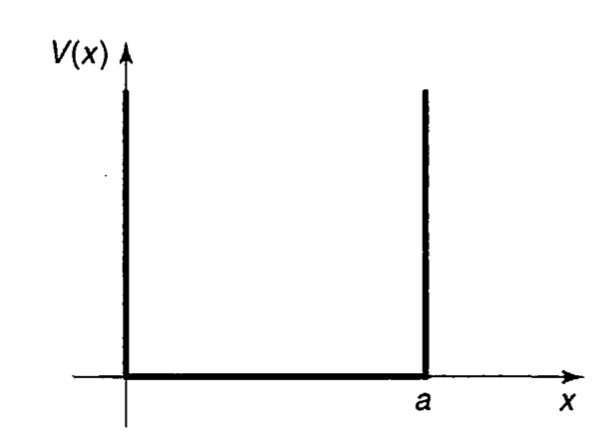
\includegraphics[scale=0.5]{fig/01.png}
		\caption{The infinte square well potential (\ref{2.19})}
		\label{fig:2.1}
	\end{center}	
\end{figure}

Suppose
\begin{equation}\label{2.19}
	V(x)=\left\{\begin{array}{lc}
		0&,0\leq x\leq a\\ \infty & \mbox{,otherwise}\end{array}
		\right.
\end{equation}
Fig. (\ref{fig:2.1}). A particle in this potential is completely free, except at two ends ($x=0$ and $x=a$), where an infinte force prevents it from escaping.

\textit{Outside} the well, $\psi(x)=0$ (the probability of findig the particle there is zero) \textit{Inside} the well, where $V=0$, the time-independent Schrodinger equation (\ref{2.5}) reads
\begin{equation}\label{2.20}
	-\frac{\hbar^2}{2m}\dv[2]{\psi}{x}=E\psi
\end{equation}
or
\begin{equation}\label{2.21}
	\dv[2]{\psi}{x}=-k^2\psi,\qquad \mbox{where } k\equiv\frac{\sqrt{2mE}}{\hbar}
\end{equation}
(By writinf it in this way, I have tacitly assumed that $E\geq 0$.) Equation (\ref{2.21}) is the classical \textbf{simple harmonic oscilaltor} equation; the general solution is
\begin{equation}\label{2.22}
	\psi(x)=A\sin kx + B\cos kx
\end{equation}
where $A$ and $B$ are arbitraty constants. Tipically, these constants are fixed by the \textbf{boundary conditions} of the problem. What are the appropiate boundary conditions for $\psi(x)$? Ordinatily, both $\psi$ and $\dd \psi/\dd x$ are continuous, but where the potential goes to infinity only the first of these applies.

Continuity of $\psi(x)$ requieres that
\begin{equation}\label{2.23}
	\psi(0)=\psi(a)=0
\end{equation}
so as to join onto the solution outisde the well. What does this tell us about $A$ and $B$? Well,
\begin{equation*}
	\psi(0)=A\sin 0+B\cos 0=B
\end{equation*}
so $B=0$, and hence
\begin{equation}\label{2.24}
	\psi(x)=A\sin kx
\end{equation}
Then $\psi(a)=A\sin ka$, so either $A=0$ (in which case we're left with the trivial --non-normalizable--solution $\psi(x)=0$), or else $\sin ka=0$, which means that
\begin{equation}\label{2.25}
	ka = 0,\pm \pi,\pm 2\pi,\pm 3\pi,...
\end{equation}
But $k=0$ is no good (again, that would imply $\psi(x)=0$),and the negative solutions give nothing new, since $\sin(-\theta)=-\sin(\theta)$ andw e can absorb the minus sign into $A$. So the \textit{distinct} solutions are
\begin{equation}\label{2.26}
	k_n=\frac{n\pi}{a},\qquad \mbox{with } n=1,2,3,...
\end{equation}
Curiously, the boundary condition at $x=a$ does not determine the constant $A$, but rather the constant $k$, and hence the possible values of $E$:
\begin{equation}\label{2.27}\marginnote{Possible values of $E$}
	\boxed{E_n=\frac{\hbar^2k_n^2}{2m}=\frac{n^2\pi^2\hbar^2}{2ma^2}}
\end{equation}
In radical contrast to the classical case, a quantum particle in the infinite square well cannot have just any old energy--it has be one of these special \textbf{allowed} values\footnote{Notice that the quantization of energy emerged as a rather technical consequence of the boudnary conditions on solutions to the time-independent Schrodinger equation}. To find $A$ we normalize $\psi$:
$$\int_a^{a}|A|^2\sin^2(kx)\dd x=|A|^2\frac{a}{2}=1,\qquad \mbox{ so  }|A|^2=\frac{2}{a}$$ 
This only determines the ,agnitude if $A$,  but it is simples to pick the positive real root: $A=\sqrt{2/a}$ (the phase of $A$ carries no physical significance anyway). Inside the well, the, the solutions are
\begin{equation}\label{2.28}
	\boxed{\psi_n(x)=\sqrt{\frac{2}{a}}\sin\left(\frac{n\pi}{a}x\right)}
\end{equation}
As a collection, the functions $\psi_n(x)$ have some interesting and important properties:
\begin{enumerate}
	\item They are alternately \textbf{even} and \textbf{odd}, with respecto to the center of the well: $\psi_1$ is even, $\psi_2$ is odd, $\psi_3$ is even,  and so on.
	\item 
		As you go up in energy, each successive state has one more \textbf{node} (zero-crossing): $\psi_1$ has one (the end points don't count), $\psi_4$ has one, $\psi_3$ has two, and so on.
	\item They are mutually \textbf{orthogonal}, in the sense that
		\begin{equation}\label{2.29}
	\int\psi_m(x)^*\psi_n(x)\dd x=0
\end{equation}
whenever $m\neq n$
We can combine orthogonality and normalization into a single satatement\footnote{In this case the $\psi$'s are real, so the * on $\psi_m$ is unnecessary, but for future purposes it's a good idea to get the habir of putting it there.}:
\begin{equation}\label{2.30}
	\boxed{\int\psi_m(x)^*\psi_n(x)\dd x=\delta_{mn}}
\end{equation}
We say that the $\psi$'s are \textbf{orthonormal}.'
\item They are \textbf{complete}, in the sense that any other function, $f(x)$, can be expressed as a linear combination of them:
	\begin{equation}\label{2.32}
	f(x)=\sum_{n=1}^\infty c_n\psi_n(x)=\sqrt{\frac{2}{a}}\sum_{n=1}^\infty c_n\sin\left(\frac{n\pi}{a}x\right)
\end{equation}
\end{enumerate}
(\ref{2.32}) is nothing but the \textbf{Fourier series} for $f(x)$, and the fact that any function can be expanded in this way is sometimes called \textbf{Dirichlet's theorem} 
The coefficients $c_n$ can be evaluated--for a given $f(x)$--by a method I call \textbf{Fourier's trick}, which beautifully exploits the orthonormality of $\{\psi_n\}$: Multiply both sides of (\ref{2.32}) by $\psi_m(x)^*$, and integrate
\begin{equation}\label{2.33}
	\psi_m(x)^*f(x)\dd x=\sum_{n=1}^\infty c_n\int\psi_m(x)^*\psi_n(x)\dd x=\sum_{n=1}^\infty c_n\delta_{nm}=c_n
\end{equation}
Thus the $n$th coefficient in the expansion of $f(x)$ is 
\begin{equation}\label{2.34}
	\boxed{c_n=\int\psi_n(x)^*f(x)\dd x}
\end{equation}
Completeness holds for all the potentials you are likely to encounter, but the proofs tens to be nasty and laborious.

The stationary states (\ref{2.18}) of the infinite square well are evidently
\begin{equation}\label{2.35}
	\Psi_n(x,t)=\sqrt{\frac{2}{a}}\sin\left(\frac{n\pi}{a}x\right)e^{-i(n^2\pi^2\hbar/2ma^2)t}
\end{equation}
I claimed (\ref{2.17}) that the most general solution to the (time-dependent) Schrodinger equation is a linear combinations of stationary states:
\begin{equation}\label{2.36}
	\Psi(x,t)=\sum_{n=1}^\infty c_n\sqrt{\frac{2}{a}}\sin\left(\frac{n\pi}{a}x\right)e^{-i(n^2\pi^2\hbar/2ma^2)t}
\end{equation}
It remaisn only for me to demosntrate that I can fit any prescribed initial wave fucntion, $\Psi(x,0)$, by appropiate choice of the coefficients $c_n$:
\begin{equation*}
	\Psi(x,0)=\sum_{n=1}^\infty c_n\psi_n(x)
\end{equation*}
The completeness of the $\psi$'s guarantees that I can always express $\Psi(x,0)$ in this way, and their orthonormality licenses the use of Fourier's trick to determine the actual coefficients:
\begin{equation}\label{2.37}
	c_n=\sqrt{\frac{2}{a}}\int_a^{a}\sin\left(\frac{n\pi}{a}x\right)\Psi(x,0)\dd x
\end{equation}
That does it: Given the initial wave function, $\Psi(x,0)$, we first compute the expansion coefficients $c_n$ using (\ref{2.37}), and the plug these into (\ref{2.36}) to obtain $\Psi(x,t)$.

Loosely speaking, $c_n$ tells you the "amount of $\psi_n$ that is contained in $\Psi$". Some people like to say that $|c_n|^2 $ is the "probability of finding the particle in the $n$th stationary state", but this is a bad language; the particle is in the state $\Psi$, not $\Psi_n$, and, anuhow, in the laboratory you don't "find a particle to be in a particular state" --you measure some observable, and what you get is a number. As we'll see next, what $|c_n|^2$ tells you is the probability that a measurement of the energy would yield the value $E_n$ (a competent measurement will always return one og the "allowed" values--hebce the name--and $|c_n|^2$ is the probability of getting the particular value $E_n$).

Of course, the sum of these probabilities shoul be $1$,
\begin{equation}\label{2.38}
	\boxed{\sum_{n=1}^\infty |c_n|^2=1}
\end{equation}
Indeed, this follows follows from the normalization of $\Psi$.

Moreover, the expectation value of the energy must be
\begin{equation}\label{2.39}\marginnote{Expectation value of the energy}
	\boxed{<H>=\sum_{n=1}^\infty |c_n|^2E_n}
\end{equation}
Notice that the probability of getting a particular energy is independent of time, and so, a fortiori, is the expectation value of $H$. This is a manifestation of \textbf{conservatio of energy} in quantum mechanics.

\section{The Harmonic Oscillator}
The paradigm for a classical harmonic oscillator is a mass $m$ attached to a spring of force constant $k$. The motion is governed by \textbf{Hooke's law}, $$F=-kx=m\dv[2]{x}{t}$$ (ignoring friction), and the solution is
$$x(t)=A\sin(\omega t)+B\cos(\omega t)$$ where
\begin{equation}\label{2.41}
	\omega \equiv\sqrt{\frac{k}{m}}
\end{equation}
is the (angular) frequency of the oscillation. The potential energy is
\begin{equation}\label{2.42}
	V(x)=\frac{1}{2}kx^2
\end{equation}
its graph is a parabola.

Virtually any oscillatory motion is approximately simple harmonic, as long as the aplitude is small.

The \textit{quantum} problem is to solve the Schrodinger equation for the potential
\begin{equation}\label{2.43}
	V(x)=\frac{1}{2}m\omega^2x^2
\end{equation}
(it it customary to eliminate the spring constant in favor of the classical frequency, using (\ref{2.41})). As we have seen, it suffices to solve the time-independent Schrodinger equation:
\begin{equation}\label{2.44}
	-\frac{\hbar^2}{2m}\dv[2]{x}{t}+\frac{1}{2}m\omega^2x^2\psi=E\psi
\end{equation}
In the literature you will find two entirely different approaches to this problem. The first is a straightforward "brute force" solution to the differential equation, usin the \textbf{power series method}; it has the virtue that the same strategy can be applied to many other potentials. The second is a diabolically clever algebraic technique, using so-called \textbf{ladder operator}. We'll se the algebraic methos first, because it is quicker and simpler (and a lot more fun)\footnote{We'll encounter some of the same strategies in the theory og angular momentum, and the technique generalizes to a broad class of potentials in \textbf{super-symmetric quantum mechanics}}. 

\subsection{Algebraic Method}\label{sec:2.3.1}
To begin with, let's rewrite (\ref{2.44}) in a more suggestive form:
\begin{equation}\label{2.45}
	\frac{1}{2m}[p^2+(m\omega x)^2]\psi=E\psi
\end{equation}
where $p\equiv (\hbar/i)\dd /\dd x$ is, of course, the momentum operator. The basic idea is to \textit{factor} the Hamiltonian,
\begin{equation}\label{2.46}
	H=\frac{1}{2m}[p^2+(m\omega x)^2]
\end{equation}
If these were \textit{numbers}, it would be easy: $$u^2+v^2=(iu+v)(-iu+v)$$
Here, however, it's not quite so simple, because $p$ and $x$ are \textit{operators},  and operators do not, in general, \textbf{commute} ($xp$ is not de same as $px$). Still, this does motivate us to examine the quantities
\begin{equation}\label{2.47}
	\boxed{a_{\pm}\equiv\frac{1}{\sqrt{2\hbar m\omega}}(\mp ip+m\omega x)}
\end{equation}
(the factor in front is just there to make the final result look nicer).

Well, what is the product $a_-a_+$?
\begin{align*}
	a_-a_+&=\frac{1}{2\hbar m\omega}(ip+m\omega x)(-ip+m\omega x)\\
				&=\frac{1}{2\hbar m\omega}[p^2+(m\omega x)^2-im\omega(xp-px)]
\end{align*}
As anticipated, there's an extra term, involving $(xp-px)$. We call this the \textbf{commutator} of $x$ and $p$; it is a measure of how badly the \textit{fail} to commute. In general the commuatator of operators $A$ and $B$ (written with brackets) is
\begin{equation}\label{2.48}
	[A,B]\equiv AB-BA
\end{equation}
In this notation,
\begin{equation}\label{2.49}
	a_-a_+=\frac{1}{2\hbar m\omega}[p^2+(m\omega x)^2]-\frac{i}{2\hbar}[x,p]
\end{equation}
We need to figure out the commuatator of $x$ and $p$. \textit{Warning}: Operators are notoriously slippery to work with in the abstract, and you are bound to make mistakes unless you give them a "test function", $f(x)$, to act on. At the end you can throw away the test function, and you'll be left with an equation involving the operators alone. In the present case we have:
\begin{equation}\label{2.50}
	[x,p]f(x)=\left[x\frac{\hbar}{i}\dv{f}{x}-\frac{\hbar}{i}\dv{xf}{x}\right]=\frac{\hbar}{i}\left(x\dv{f}{x}-x\dv{f}{x}-x\right)=i\hbar f(x)
\end{equation}
Dropping the test function, which has served its purpose,
\begin{equation}\label{2.51}\marginnote{Cannonical commutation relation}
	\boxed{[x,p]=i\hbar}
\end{equation}
This lovely and obiquitous result is known as the \textbf{cannonical commutation relation}\footnote{In deep sense all of the mysteries of quantum mechanics can be traced to the fact that position and momentum do not commute. Indeed, some authors take the cannoncial commuation relation as an \textit{axiom} of the theory, and use ir to \textit{derive} $p=(\hbar/i)\dd/\dd x$}.

With this, (\ref{2.49}) becomes

\begin{equation}\label{2.52}
	a_-a_+=\frac{1}{\hbar\omega}H+\frac{1}{2}
\end{equation}
or
\begin{equation}\label{2.53}
	H=\hbar\omega\left(a_-a_+-\frac{1}{2}\right)
\end{equation}
Evidently the Hamiltonian does not factor perfectly--there's that extra $-1/2$ on the right. Notice that the orderinf of $a_+$ and $a_-$ is important here; the same argument, with $a_+$ on the left, yields
\begin{equation}\label{2.54}
	a_+a_-=\frac{1}{\hbar\omega}H-\frac{1}{2}
\end{equation}
In particular,
\begin{equation}\label{2.55}
	[a_-,a_+]=1
\end{equation}
So the Hamiltonian can equally well be written
\begin{equation}\label{2.56}
	H=\hbar\omega\left(a_+a_-+\frac{1}{2}\right)
\end{equation}
In terms of $a_{\pm}$, then, the Schrodinger equation\footnote{I'm getting tired of writing "time-independent Schrodinger equation", so when it's clear from the context which one I mena, I'll just call it the "S equation".} for the harmonic oscilaltor takes the form
\begin{equation}\label{2.57}
	\hbar\omega\left(a_{\pm}a_{\mp}\pm\frac{1}{2}\right)\psi=E\psi
\end{equation}
(in equations like this you rrad the upper signs all the way across, or else the lower signs).

Now, here comes the crucial step: I claim that if \textit{$\psi$ satisfies the Schrodinger equations with enrgy $E$, (that is: $H\psi=E\psi$), then $a_+\psi$ satisfies the Schrodinger equations with energy ($E+\hbar\omega$):$H(a_+\psi)=(E+\hbar\omega)(A_+\psi)$ }

By the same token, $a_-\psi$ is a solution with energy $(E-\hbar\omega)$
\begin{align*}
	H(a_+\psi)&=(E+\hbar\omega)(a_+\psi
	H(a_-\psi)&=(E-\hbar\omega)(a_-\psi)
\end{align*}

Here, then is a wonderful machine for generating new solution, with higer and lower energies--if we could just find \textit{one} solution, to ger started! We call $a_{\pm}$ \textbf{ladder operators}, because they allow us to climb up and doen in energy; $A_+$ is the \textbf{raising operator}, and $a_-$ the \textbf{lowering operator}. 

But wait! What if I apply the lowering operator repeatedly? Eventually I'm going to reach a state with energy less than zero, which does not exist! At some point the machine must fail. How can that happen?  We know that $a_-\psi$ is a new solution to the Schrodinger equation, but \textit{there is no guarantee that it will be normalizable}--it might be zero, or its square-integral might be infinite. In practice it is the forme: There occurs a "lowest rung" (call it $\psi_0$) such that
\begin{equation}\label{2.58}
	a_-\psi_0=0
\end{equation}
We can use this to determine $\psi_0(x)$:
$$\frac{1}{\sqrt{2\hbar m\omega}}\left(\hbar\frac{\dd}{\dd x}+m\omega x\right)\psi_0=0$$ or $$\dv{\psi_0}{x}=-\frac{m\omega}{\hbar}x\psi_0$$
The differential equation is easy to solve:
$$\int\frac{\dd \psi_0}{\psi_0}=-\frac{m\omega}{\hbar}\int x\dd x\quad\Rightarrow\quad \ln\psi_0=-\frac{m\omega}{2\hbar}x^2+\mbox{ constant}$$ so $$\psi_0(x)=Ae^{-\frac{m\omega}{2\hbar}x^2}$$
We might as well normalize it right away: $$=|A|^2\int_{-\infty}^\infty e^{-m\omega x^2/\hbar}\dd x=|A1|^2\sqrt{\frac{\pi\hbar}{m\omega}}$$ so $A^2=\sqrt{m\omega/\pi\hbar}$, and hence
\begin{equation}\label{2.59}
	\boxed{\psi_0(x)=\left(\frac{m\omega}{\pi\hbar}\right)^{1/4}e^{-\frac{m\omega}{2\hbar}x^2}}
\end{equation}
To determine the energy of this satte we plug it into the Schrodinger equation (in the form of (\ref{2.57})), $\hbar\omega(a_+a_-+1/2)\psi_0=E_0\psi_0$. and exploit the fact that $a_-\psi_0=0$:
\begin{equation}\label{2.60}
	E_0=\frac{1}{2}\hbar\omega
\end{equation}
With our foot now securely planted on the bottom rung (the ground state of the quantum oscillator), we simply apply the raising operator (repeatedly) to generate the excited states, increasing the energy by $\hbar\omega $ with each step:
\begin{equation}\label{2.61}
	\boxed{\psi_n(x)=A_n(a_+)^n \psi_0(x),\qquad\mbox{ with  }E_n=\left(n+\frac{1}{2}\right)\hbar\omega     }
\end{equation}
where $A_n$ is the normalization constant. By applying the raising operator (repeatedly) to $\psi_0$, then, we can (in principle) construct all the stationary states of the harmonic oscillator. Meanwhile, without ever doing that explicitly, we have determined the allowed energies.

You can even get the normalization algebraically, but it takes some fancy foorwork, wo watch closely. we know that $a_{\pm}\psi_n$ is \textit{proportional} to $\psi_{m\pm 1}$,
\begin{equation}\label{2.63}
	a_+\psi_n=c_n\psi_{n+1},\qquad a_-\psi_n=d_n\psi_{n-1}	
\end{equation}
but what are the proportionality factors, $c_n$ and $d_n$? First note that for "any" functions $f(x)$ and $g(x)$,
\begin{equation}\label{2.64}
	\int_{-\infty}^\infty f^*(a_{\pm}g)\dd x=\int_{-\infty}^\infty (a_{\mp}f)^*g\dd x
\end{equation}
(In the language of linear algebra, $a_{\mp}$ is the \textbf{hermitian conjuagte} of $A_{\pm}$).
In particular, $$\int_{-\infty}^\infty (a_{\pm}\psi_n)^*(a_{\pm}\psi_n)\dd x=\int_{-\infty}^\infty(a_{\mp}a{\pm}\psi_n)^*\psi_n\dd x $$ But (invoking (\ref{2.57}) and (\ref{2.61}))
\begin{equation}\label{2.65}
	a_+a_-\psi_n=n\psi_n,\qquad a_-a_+\psi_n=(n+1)\psi_n
\end{equation}
so
$$\int_{\infty}^\infty(a_+\psi_n)^*(a_+\psi_n)\dd x=|c_n|^2\int_{-\infty}^\infty |\psi_{n+1}|^2\dd x=(n+1)\int_{-\infty}^\infty |\psi_n|^2\dd x $$
$$\int_{-\infty}^\infty(a_-\psi_n)^*(a_-\psi_n)\dd x=|d_n|^2\int_{-\infty}^\infty |\psi_{n-1}|^2\dd x=n\int_{-\infty}^\infty |\psi_n|^2\dd x $$
But since $\psi_n$ and $\psi_{n\pm 1}$ are normalized, it follows that $|c_n|^2=n+1$ and $|d_n|^2=n$ and hence.
\begin{equation}\label{2.66}
	\boxed{a_+\psi_n\sqrt{n+1}\psi_{n+1},\qquad a_-\psi_n=\sqrt{n}\psi_{n-1}}
\end{equation}
Thus
$$\psi_1=a_+\psi_0,\qquad \psi_2=\frac{1}{\sqrt{2}}a_+\psi_1=\frac{1}{\sqrt{2}}(a_+)^2\psi_2$$
$$\psi_3=\frac{1}{\sqrt{3}}a_+\psi_2=\frac{1}{\sqrt{3\cdot 2}}(a_+)^3\psi_0,\qquad \psi_4=\frac{1}{\sqrt{4}}a_+\psi_3=\frac{1}{\sqrt{4\cdot 3\cdot 2}}(a_+)^4\psi_0$$
and so on .Clearly
\begin{equation}\label{2.67}
	\boxed{\psi_n=\frac{1}{\sqrt{n!}}(a_+)^n\psi_o}
\end{equation}
which is to say that the normalization factor in (\ref{2.61}) is $A_n=1/\sqrt{n!}$ .

As in the case of the infinite square well, the stationary states if the harmonic oscillator are orthogonal:
\begin{equation}\label{2.68}
	\int_{-\infty}^\infty \psi_m^*\psi_n\dd x=\delta_{mn}
\end{equation}
This can be proved usign (\ref{2.65}) and (\ref{2.64}) twice--fist moving $a_+$ and then moving $a_-$:
\begin{align*}
	\int_{-\infty}^\infty \psi_m^*(a_+a_-)\psi_n\dd x&=n\int_{-\infty}^\infty\psi_m^*\psi_n\dd x\\
																									 &=\int_{-\infty}^\infty(a_-\psi_m)^*(a_-\psi_n)\dd x=\int_{-\infty}^\infty(a_-a_-\psi_m)^*\psi_n\dd x\\
																									 &=m\int_{-\infty}^\infty\psi_m^*\psi_n\dd x
\end{align*}
Unless $m=n$, then, $\int\psi_m^*\psi_n\dd x$ must be zero. Orthonomality means that we can again use Forier's trcik (\ref{2.34}) to evaluate the coefficients, when we expand $\Psi(x,0)$ as a linear combination of stationary states (\ref{2.16}), and $|c_n|^2$ is again the probability that a measurement of energy would yield the vakue $E_n$.

\subsection{Analytic Method}
We return now to the Schrodinger equation for the harmonic oscillator,
\begin{equation}\label{2.70}
	-\frac{\hbar^2}{2m}\dv[2]{\psi}{x}+\frac{1}{2}m\omega^2x^2\psi=E\psi
\end{equation}
and solve it directly, by the series method. Thing loock a little cleanes if we introduce the dimensionless variable
\begin{equation}\label{2.71}
	\xi\equiv\sqrt{\frac{m\omega}{\hbar}}x
\end{equation}
in terms of $\xi$ the Schrodinger equation reads
\begin{equation}\label{2.72}
	\dv[2]{\psi}{\xi}=(\xi^2-K)\psi
\end{equation}
where $K$ is the energy, in units of $(1/2)\hbar\omega$:
\begin{equation}
	k\equiv\frac{2E}{\hbar\omega}
\end{equation}
Our problem is to solve (\ref{2.72}), and in the process obtain the "allowed" values of $K$ (and hence of $E$).

To begin with, note that at very large $\xi$ (which is to say, at very large $x$), $\xi^2$ completely dominates over the constant $K$, so in this regime
\begin{equation}\label{2.74}
	\dv[2]{\psi}{\xi}\approx \xi^2\psi
\end{equation}
which has the approximate solution
\begin{equation}\label{2.75}
	\psi(\xi)\approx Ae^{-\psi^2/2}+Be^{+\xi^2/2}
\end{equation}
The $B$ term is clearly not normalizable (it blows up as $|x|\to\infty)$; the physucally acceptable solutions, then, have the asympotic form
\begin{equation}\label{2.76}
	\psi(\xi)\to ()e^{-\xi^2/2},\qquad \mbox{ at large $\xi$ }
\end{equation}
This suggests that we "peel off" the exponential part,
\begin{equation}\label{2.77}
	\psi(\xi)=h(\xi)e^{-\xi^2/2}
\end{equation}
in hopes that what remains, $h(\xi)$, has a simplier functional form than $\psi(\xi)$ itself. Differentiating (\ref{2.77})
$$\dv{\psi}{\xi}=\left(\dv{h}{\xi}-\xi h\right)e^{-\xi^2/2}$$ and
$$\dv[2]{\psi}{\xi}=\left(\dv[2]{h}{\xi}-2\xi\dv{h}{\xi}+(\xi^2-1)h\right)e^{-\xi^2/2}$$
so the Schrodinger equation (\ref{2.72}) becomes
\begin{equation}\label{2.78}
	\dv[2]{h}{\xi}-2\xi\dv{h}{\xi}+(K-1)h=0
\end{equation}
I propose to look fot solutions to (\ref{2.78}) in the form of \textit{power series} in $\xi$\footnote{This is known as the \textbf{Frobenius method} for solving a differential equation. According yo Taylor's theorem, any reasonably well-behaven function can be expressed as a power series, so (\ref{2.79}) ordinarily involver no loss of generality.}:
\begin{equation}\label{2.79}
	h(\xi)=a_0+a_1\xi+a_2\xi^2+\cdots =\sum_{j=0}^\infty a_j\xi^j
\end{equation}
Differentiating the seris term by term, $$\dv{h}{\xi}=a_1+2a_2\xi+3a_3\xi^2+\cdots =\sum_{j=0}^\infty ja_j\xi^{j-1}$$
and $$\dv[2]{h}{\xi}=2a_2+2\cdot 3a_3\xi +3\cdot 4a_4\xi^2+\cdots =\sum_{j=0}^\infty (j+1)(j+2)a_{j+2}\xi^j$$
Putting these into (\ref{2.78}), we find
\begin{equation}\label{2.80}
	\sum_{j=0}^\infty [(j+1)(j+2)a_{j+2}-2ja_j+(K-1)a_j]\xi^j=0
\end{equation}
It follows (from the uniqueness of power series expansions) that the coefficient of \textit{each power} of $\xi$ must vanish, $$(j+1)(j+2)a_{j+1}-2ja_j+(K-1)a_j=0$$ and hence that
\begin{equation}\label{2.81}
	a_{j+2}=\frac{(2j+1-K)}{(j+1)(j+2)}a_j
\end{equation}
This \textbf{recursion formula} is enterely equivalent to the Schrodinger equation. Starting with $a_0$, it generates all the even-numbered coefficients
$$a_2=\frac{(a-K)}{2}a_0\quad a_4=\frac{(5-K)}{12}a_2=\frac{(5-K)(1-K)}{24}a_0,\quad \cdots $$
and starting with $a_2$, it generates the odd coefficients: $$a_3=\frac{(3-K)}{6}a_1,\quad a_5=\frac{(7-K)}{20}a_3=\frac{(7-K)(3-K)}{120}a_1,\quad \cdots $$
We write the complete solution as
\begin{equation}\label{2.82}
	h(\xi)=h_{\mbox{even}}(\xi)+h_{\mbox{odd}}(\xi)
\end{equation}
where $$h_{\mbox{even}}(\xi)\equiv a_0+a_2\xi^2+a_4\xi^4+\cdots $$ is an even fucntion of $\xi$, built on $a_0$, and $$h_{\mbox{odd}}(\xi)\equiv a_1\xi+a_3\xi^3+a_5\xi^5+\cdots $$ is an odd function, built on $a_1$
(\ref{2.81}) determines $h(\xi)$ in terms of two arbitrary constants ($a_0$ and $a_1$)--which is just what we would expect, for a second-order differentual equation.

However, not all the solutions so obtained are \textit{normalizable}. Fot at very large $j$, the recursion formula becomes (approximayely) $$a_{j+2}\approx \frac{2}{j}a_j$$ with the (approximate) solution $$a_j\approx\frac{C}{(j/2)!}$$ for some constant $C$, and this yields (at large $\xi$, where the higher powers dominate) $$h(\xi)\approx C\sum\frac{1}{(j/2)!}\xi^j\approx C\sum\frac{1}{j!}\xi^{2j}\approx Ce^{\xi^2}$$ Now, if $h$ goes like $\exp(\xi^2/2)$, then $\psi$ (remember $\psi$?--that's what we're trying to calculate) goes like $\exp(\xi^2/2)$ (\ref{2.77}), which is precisely the asymtotic behavior we didn's want\footnote{It's no surprise that the ill-behaven solutions are still in (\ref{2.81}):this recursion relation is equivalent to the Schrodinger equation, so it's got to include both the asymtotic forms we found in (\ref{2.75})}. There is only one way to wiggle out of this: For normalziable solutions the \textit{power series must terminate}. There must occur some "highest" $j$ (call it $n$), such that the recursion formula spits out $a_{a+2}=0$ (this woll truncate either series $h_{\mbox{even}}$ or the series $h_{\mbox{odd}}$; the other one must be zero from that start: $a_1=0$ if $n$ is even, and $a_0=0$ if $n$ is odd). For physically acceptable solutions, then, (\ref{2.81}) requires that $$K=2_n+1$$ for some non-neagtive integer $n$, which is to say (referring to (\ref{2.77})) that the \textit{energy} must be
\begin{equation}\label{2.83}
	E_n=\left(n+\frac{1}{2}\right)\hbar\omega,\qquad \mbox{ for $n=0,1,2,...$ }
\end{equation}
Thus we recover, by a completely different method, the fundamental quantization condition we found algebraically in (\ref{2.61}).










%\chapter{Formalism}
\section{Hilbert Space}

The purpose of this chapter is to recast the theory in a more powerful form.

Quantum theory is based on two constructs: \textit{wave functions} and \textit{operators}. The state of a system is represented by its wave function, obervables are represented by operators. Mathematically, weave functions satify the defining conditions for abstract \textbf{vectors}, and operators act on them as \textbf{linear transformations}. So the natural language of quantum mechanics is \textbf{linear algebra}.

But it is not, I suspect, a form of linear algebra with which you are immediately familiar. In an $N$-dimensional space it is simplest to represent a vector $\ket{\alpha}$, by the $N$-tuple of its components, $\{a_n\}$, with respect to a specified orthonormal basis:
\begin{equation}\label{3.1}
	\ket{\alpha}\to\vb*{a}=\mqty(a_1\\a_2\\\vdots \\a_N)
\end{equation}
The \textbf{inner product}, $\braket{\alpha}{\beta}$, of two vectors (generalizng the dot product in three dimensions) is the complex numebr,
\begin{equation}\label{3.2}
	\braket{\alpha}{\beta}=a_1^*b_1+a_2^*b_2+\cdots +a_N^*b_N
\end{equation}
Linear transformations, $T$, are represented by \textbf{matrices} (with respect to the specified basis), which act on vectors (to produce new vectors) by the ordinary rules of matrix multiplication:
\begin{equation}\label{3.3}
	\ket{\beta}=T\ket{\alpha}\to \vb{b}=\vb{T}\vb{a}=\mqty(t_{11}&t_{12}&\cdots & t_{1N}\\
	t_{21}&t_{22}&\cdots&t_{2N}\\
	\vdots&\vdots&\vdots&\vdots\\
	t_{N1}&t_{N2}& \cdots &t_{NN})
\end{equation}
But the "vectors" we encounter in quantum mechanics are (for the most specified) \textit{functions}, and they live in infinite-dimensional spaces. For them the $N$-tuple/matrix notation is awkward, at best, and manipulations that are well-behaved in the finite dimensional case can be problematic. (The underlying reason is that whereas the finite sum in (\ref{3.2}) always exists, an infinite sum--or a integral-- may not converge, in which case the inner product does not exists, and any argument involving inner products is immediately suspect.).

The collection of all functions of $x$ constitutes a vector space, but fot our purposes it is much too latge. To represent a possible physical state, the function $\Psi$ must be normalized:
$$\int |\Psi|^2\dd x=1$$ The set of all \textbf{square-integrable functions}, on a specified ineterval\footnote{Fot is, the limits ($a$ and $b$) will almost always be $\\pm\infty$, but we might as well keep thing more general for the moment},
\begin{equation}\label{3.4}
	f(x)\qquad \mbox{ such that  }\qquad \int_a^b |f(x)|^2\dd x<\infty
\end{equation}
constitutes a (much smaller) vector space. Mathematicians call it $L_2(a,b)$; physicist call it \textbf{Hilbert space}. In quantum mechanics then
\begin{equation}\label{3.5}
	\boxed{\mbox{\textbf{Wave functions live in Hilbert space.}}}
\end{equation}
We define the \textbf{inner product of two functions}, $f(x)$ and $g(x)$, as follows:
\begin{equation}\label{3.6}
	\braket{f}{g}\equiv\int_a^b f(x)^*g(x)\dd x
\end{equation}
If $f$ and $g$ are both square-integrable (that is, if they are both in hilber spaces), their inner product is guaranteed to exist. This follows from the integral \textbf{Schwartz inequality}:
\begin{equation}\label{3.7}
	\left|\int_a^bf(x)^*g(x)\dd x\right|\leq \sqrt{\int_a^b|f(x)|^2\dd x\int_a^b|g(x)|^2\dd x}
\end{equation}
Notice in particular that
\begin{equation}\label{3.8}
	\braket{g}{f}=\braket{f}{g}^*
\end{equation}
Moreover, the inner product of $f(x)$ with itself,
\begin{equation}\label{3.9}
	\braket{f}{f}=\int_a^b|f(x)|^3\dd x
\end{equation}
is real and and non-negative; it's zero only when $f(x)=0$. 

A function is said to be \textbf{normalized} if its inner product with itself is $1$; two functions are \textbf{orthogonal} of their inner product is $0$; and a set of functions, $\{f_n\}$, is \textbf{orthonormal} of they are normalized and mutually orthogonal
\begin{equation}\label{3.10}
	\braket{f_m}{f_n}=\delta_{mn}
\end{equation}
Finally, a set of functions is \textbf{compelte} if any other function (in Hilbert space) can be expreded as a linear combination of them:
\begin{equation}\label{3.11}
	f(x)=\sum_{n=1}^\infty c_nf_n(x)
\end{equation}
If rge functuons $\{f_n(x)\}$ are orthonrmal, the coefficients are given by Fourier's trick
\begin{equation}\label{3.12}
	c_n=\braket{f_n}{f}
\end{equation}

\section{Obervables}
\subsection{Hermitian Operators}
The expectation value of an observable $Q(x,p)$ can be expressed very neatly in inner-product notation:
\begin{equation}\label{3.13}
	<Q>=\int \Psi^*\hat{Q}\Psi\dd x=\bra{\Psi}\ket{\hat{Q}\Psi}
\end{equation}
Now, the outcome of a measurement has got to be \textit{real}, and so, a fortiori, is the average of many measurements:
\begin{equation}\label{3.14}
	<Q>=<Q>^*
\end{equation}
But the complex conjugate of an inner product reverses the order (\ref{3.8}), so
\begin{equation}\label{3.15}
	\bra{\Psi}\ket{\hat{Q}\Psi}=\bra{\hat{Q}\Psi}{\ket\Psi}
\end{equation}
and this must hold true for any wave function $\Psi$. Thus operators representing \textit{obervables} have the very special property that
\begin{equation}\label{3.16}
	\bra{f}\ket{\hat{Q}f}=\bra{\hat{Q}f}\ket{f}\qquad\mbox{for all $f(x)$}
\end{equation}
We call such operators \textbf{hermitian}.

The essentiak point is that a hermitian operator can be applied either to the first member of an inner product or to the second, with the same result, and hermitian operators naturally arise in quantum mechanics because their expectations values are real:
\begin{equation}\label{3.18}
	\boxed{\mbox{\textbf{Obervables are represented by hermitian operators.}}}
\end{equation}
Is the momentum operator, for example, hermitian?
\begin{equation}\label{3.19}
	\bra{f}\ket{\hat{p}g}=\int_{-\infty}^\infty \frac{\hbar}{i}\dv{g}{x}\dd x=\frac{\hbar}{i}\eval{f^*g}_{-\infty}^\infty +\int_{-\infty}^\infty \left(\frac{\hbar}{i}\dv{f}{x}\right)^*g\dd x=\bra{\hat{p}f}\ket{g}
\end{equation}
Notice if $f(x)$ and $g(x)$ are squared integrable, they must go to zero at $\pm\infty$.

\subsection{Determinate States}
Ordinarily, when you measure an obervable $Q$ on an ensamble of identically prepared system, all in the same state $\Psi$, you do not ger the same reuslt each time--this is the indeterminancy of quantum mechanics. \textit{Question:} Would it be possible to prepare a state such that \textit{every} measurement of $Q$ is certain to return the \textit{same} value (call it $a$)? This would be, if younlike, a \textbf{determinate state}, for the obervable $Q$ (Actually, we already know one example: Stationary states are dterminate states of Hamiltonian; a measurement of the total enery, on a particle in the stationary state $\Psi_n$, is certain to yield the corresponding "allowed" energy $E_n$).

Well, the standard deviation of $Q$, in a determiante state, would to be zero, shich is to say,
\begin{equation}\label{3.21}
	\sigma^2=<(\hat{Q}-<Q>)^2>=\bra{\Psi}\ket{(\hat{Q}-q)^2\Psi}=\bra{(\hat{Q}-q)\Psi}\ket{(\hat{Q}-q)\Psi}=0
\end{equation}
But the only function whose inner product with itself vanishes is $0$, so
\begin{equation}\label{3.22}
	\hat{Q}\Psi=q\Psi
\end{equation}
This is the \textbf{eigenvalue equation} for the operator $\hat{Q}$; $\Psi$ is an \textbf{eigenfunction} of $\hat{Q}$, and $q$ is the corresponding \textbf{eigenvalue}. Thus
\begin{equation}\label{3.23}
	\boxed{\mbox{\textbf{Determiante states are eigenfunctions of }$\hat{Q}$}}
\end{equation}
Measurements of $Q$ a¡on such states is certain to yield the eigenvalue, $q$.

Note that the eigenvalue is a number (not a operator or a function). You can multuply any eigenfunction by a constant,  and it is still an eigenfunction, with the same eigenvalue. Zero does not count as an eigenfunction. But there's nothing wrong with zero as an eigenvalue. The collection of all the eigenvalues of an operator is called its \textbf{specturm} . Sometimes two (or more) linearly independent eigenfunctions share the same eigenvalue; in that case the spectrum is said to be \textbf{degenerate}.

\section{Eigenfunctions of a Hermitian Operator}
Our attention is thus directed to the \textit{eigenfunction of hermitian operators} (physically: determine states of obervables). These fall into two categories: If the spectrum is \textbf{discrete} (i.e., the eigenvalues are separated from one another) then the eigenfunctions lie in Hilbert space and they constitute physically realizable states. If the spectrum is \textbf{contonuous} (i.e., the eigenvalues fill out an entire range) then the eigenfunctions are non normalizable, and they do not represent possible wave functions (\textit{though linear cominations} of them--involving neccessarily a spread in eigenvalues--may be normalizable). Some operator have a discrete spectrum only (for example, the Hamiltonian for the harmonic oscillator). some have only a continuous spectrum (for example, the free partivle Hamiltonian), and some have both discrete part and a continuous part (for example, the Hamiltonian for a finite square well). The discrete case is easier to handle. because the relevant inner product are guaranteed to exist--in fact, it is very similar to the finite-dimensional theory (the eigenvectors of a hermitian matrix). I'll treat the discrete case first, and then the continuous one:

\subsection{Discrete Spectra}
Mathematically, the normalizable eigenfunctions of a hermitian have two important properties:
\begin{teo}
	Their \textit{eqigenvalues} are \textit{real}.
\end{teo}
This is comforting: If you measure an obervable on a particle ina  dterminate state, you will at leat least get a real number.
\begin{teo}
	Eigenfunctions belonging to distinct eigenvalues are \textit{orthogonal}.
\end{teo}
In  a \textit{finite}-diemsnional vector space the eigenvectos of a hermitian matrix have a third fundamental property: The span the space (every vector can be expressed as a linar combination of them). Unfortunately, the proof does not generalize to infinite-dimensional spaces. But the property itslef is essential to the internal consistency of quantum mechanics, so we will take it as an \textit{axiom} (or, more precisely, as a restriction on the class of hermitian operators that can represent obervables):
\begin{axiom}
	The eigenvalues of an obervable operator are \textit{compelte}: Any function (in Hilber space) can be expressed as a linear combination of them.
\end{axiom}

\subsection{Continuous Spectra}
If the spectrum of a hermitian operator is \textit{continuous}, the eigenfunctions are not normalizable, and the proofs of Theorems 1 and 2 fail, because the inner products may not exists. Nevertheless, there is a sense in which the three essential properties (reality, orthogonality, and complereness) still hold. I think it's best to approach this subtle case through specific examples.

\begin{example}
	Find the eigenfunctions and eigenvalues of the momentum operator
\end{example}
\begin{sol}
\end{sol}
Let $f_p(x)$ be the eigenfunction and $p$ the eigenvalue:
\begin{equation}\label{3.30}
	\frac{\hbar}{i}\frac{\dd}{\dd x}f_p(x)=pf_p(x)
\end{equation}
The general solution is $$f_p(x)=Ae^{ipc/\hbar}$$ This is not square-integrable, for any (complex) value of $p$--the momentum operator has no eigenfunctions in Hilbert space. And yet, if we restrict ourselves to \textit{real} eigenvalues. we do recover a kind of \textit{ersatz} "orthonormality". ...

\subsection{Generalized Statistical Interpretation}
\textbf{Generalized statistical interpretation:} If you measure an obervable $Q(x,p)$ on a particle in the state $\Psi(x,t)$, you are certain to get \textit{one of the eigenvalues} of the hermitian operator $\hat{q}(x,-i\hbar\dd/\dd x)$. If the spectrum of $\hat{Q}$ is discrete, the probability of getting the particular eigenvalue $q_n$ associated with the orthonormalized eifengunction $f_n(x)$ is
\begin{equation}\label{3.43}
	|c_n|^2,\qquad \mbox{where }\qquad c_n=\braket{f_n}{\Psi}
\end{equation}
If the sprectrum is continuous, with real eigenvalues $q(z)$ and associated Dirac-orthonormalized eigenfunctions $f_z(x)$, the probability of gettin a result in the range $\dd z$ is
\begin{equation}\label{3.44}
	|c(z)|^2\dd z \mbox{where }\qquad c(z)=\braket{f_z}{\Psi}
\end{equation}
Upon measurement, the wave function "collapses" to the corresponding eigenstate.

The statistical interpretation is raadically different from anything we encounter in classical physics. A somewhat different persperctive helps to make it plausible:
The eigenfunctions of an observable operator are \textit{complete}, so the wave function can be written as a linear combination of them:
\begin{equation}\label{3.45}
	\Psi(x,t)=\sum_nc_nf_x(x)
\end{equation}
(For simplicity, I'll assume that the spectrum is discrete; it's easy to generalise this argument to the continuous case.) Because the eigenfucntions are \textit{orthonormal}, the coefficients are given by Fourier's trick:
\begin{equation}\label{3.46}
	c_n=\braket{f_n}{\Psi}=\int f_n(x)^*\Psi(x,t)\dd x
\end{equation}
Qualitatively, $c_n$ tells you "how much $f_n$ is contained in $\Psi$", and given that a mesuremnet has to return one of the eigenvalues of $\hat{Q}$, it seems reasonable that the probability of getting the particular eigenvalue $q_n$ would be determined by the "amount of $f_n$" in $\Psi$. But because probabilities are determined by the absolute square of the wave function, the precise measure is actually $|c_n|^2$. That's the essential burden of the generalized statistical interpretation.

Of course, the total probability (summed over all outcomes) has got to be one:
\begin{equation}\label{3.47}
	\sum_n|c_n|^2=1
\end{equation}
Similarly, the expectation value of $Q$ should be the sum over all possibles outcomes of the eigenvalue times the probability of getting the eigenvalue:
\begin{equation}\label{3.49}
	<Q>=\sum_nq_n|c_n1^2
\end{equation}
The \textbf{momentum space wave function}, $\Phi(p,t)$. It is essentially the \textit{Fourier transform} of the (\textbf{position space}) wave function $\Psi(x,t)$--which, by Plancherel'stheorem, is its \textit{inverse} Fourier transform:
\begin{equation}\label{3.54}
\Phi(p,t)=\frac{1}{\sqrt{2\pi\hbar}}\int_{-\infty}^\infty e^{-ipx/\hbar}\Psi(x,t)\dd x
\end{equation}
\begin{equation}\label{3.55}
	\Psi(x,t)=\frac{1}{\sqrt{2\pi\hbar}}\int_{-\infty}^\infty e^{ipx/\hbar}\Phi(p,t)\dd p
\end{equation}
According to the generalized statistical interpretationm, the probability that a measurement of momentum would yiled a result in the range $\dd p$ is
\begin{equation}\label{3.56}
	|\Phi(p,t)|^2\dd p
\end{equation}

\section{The Uncertaintly Principle}

\section{Dirac Notation}
Imagine an ordinary vactor $\vb{A}$ in two dimensions. How would you describe this vector to someone? The most convenient way is to set up catesian axes, $x$ and $y$, and specify the components of $\vb{A}$: $a_x=\hat{i}\cdot \vb{A}, A_y=\hat{j}\cdot \vb{A}$. Of course, your sister might have drawn a different set of axed, $x'$ and $y'$, and she would report differen components: $A'_x=\hat{i}'\cdot\vb{A}, A'_y=\hat{j}'\cdot\vb{A}$. But it's all the same vector--we're simply expressing it with respecto to two different bases ($\{\hat{i},\hat{j}\}$ and $\{\hat{i}',\hat{j}'\})$. The vector itself lives "out there is space", independent of anybody's (arbitraty) choice of coordinates.

The same is true for the state of a system in quantum mechancis. It is represented by a vector, $\ket{s(t)}$, that lives "out there in Hilbert space", but we can express it with respceto to any number of different bases. The wave function $\Psi(x,t)$ is actually the coefficient in the expansion of $\ket{s(t)}$ in the basis of position eigenfunctions:
\begin{equation}\label{3.75}
	\Psi(x,t)=\braket{x}{s(t)}
\end{equation}
(with $\ket{x}$ standing fot the eigenfucntions of $\hat{x}$ with eigenvalue $x$), whereas the momentum sapce wavefunction $\Phi(x,t)$ is the expansion of $\ket{s}$ in the absis of momentum eigenfucntions:
\begin{equation}\label{3.76}
	\Phi(p,t)=\braket{p}{s(t)}
\end{equation}
(with $\ket{p}$ standing for the eigenfunction of $\hat{p}$ with eigenvalue $p$). Or we could expand $\ket{s}$ in the basis of energy eigenfunctions (supposing for simplicity that the spectrum is discrete):
\begin{equation}\label{3.77}
	c_n(t)=\braket{n}{s(t)}
\end{equation}
(with $\ket{n}$ standing for thr $n$th eigenfunction of $\hat{H}$)--(\ref{3.46}). But it's all the same state; the functions $\Psi$ and $\Phi$, and the collection of coefficients $\{c_n\}$, contain exactly the same information--they are simply three different ways of describing the same vector:
\begin{align}
	\nonumber \Psi(x,t)&=\int\Psi(y,t)\delta(x-y)\dd y=\int\Phi(p,t)\frac{1}{\sqrt{2\pi\hbar}}e^{ipx/\hbar}\dd  p\\
										 &=\sum c_ne^{-iE_nt/\hbar}\psi_n(x)\label{3.78}
\end{align}
Operators (representing obervables) are linear transformations--they "transform" one vector into another:
\begin{equation}\label{3.79}
	\ket{\beta}=\hat{Q}\ket{\alpha}
\end{equation}
Just as vectors are represented, with respect to a particular basis $\{\ket{e_n}\}$\footnote{I'll assume the basis is discrete: otherwise $n$ becomes a continuous index and the syms are replaced by integrals}, by their components,
\begin{equation}\label{3.80}
	\ket{\alpha}=\sum_n a_n\ket{e_n}, \mbox{with } a_n=\braket{e_n}{\alpha}:\quad \beta=\sum_n b_n\ket{e_n}, \mbox{with } b_n=\braket{e_n}{\beta}
\end{equation}
operators are represented (with respect to a particular basis) by their \textbf{matrix elements}\footnote{Tjis terminology is inspired, obviously, by the finite-dimensinal case, but the "matrix" will now typically have an infinite (maybe even uncountable) number of elements.}
\begin{equation}\label{3.81}
	\mel{e_m}{\hat{Q}}{e_n}\equiv Q_{mn}
\end{equation}
In this notations (\ref{3.79}) takes the form
\begin{equation}\label{3.82}
	\sum_nb_n\ket{e_n}=\sum_na_n\hat{Q}\ket{e_n}
\end{equation}
or, taking the inner product with $\ket{e_m}$,
\begin{equation}\label{3.83}
	\sum_n b_n\braket{e_m}{e_n}=\sum_na_n\mel{e_m}{\hat{Q}}{e_n}
\end{equation}
and hence
\begin{equation}\label{3.84}
	b_m=\sum_nQ_{mn}a_n
\end{equation}
Thus the matrix elements tell you how the components transform. 

Later on we will encounter sysrem that admit only a finite number ($N$) of linearly independet states. In that case $\ket{s(t)}$ lives un an $N$-dimensional vector space; it can be represented as a column of ($N$) components (with respecto to a given bases), and operators take the form of ordinary ($N\times N$) matrices. These are the simplest quantum systems--none of the subtleties associted with infinite-dimensional vector spaces arise. 

Dirac proposed to chop the bracket notation for the inner product, $\braket{\alpha}{\beta}$, into two pieces, which he called \textbf{bra}, $\bra{\alpha}$, and \textbf{ket} $\ket{\beta}$. The latter is a vector, but what exactly is the former? It's a \textit{linear function} of vectors, in the sense that when it hits a vector (to its right) it yields a (complex) number--the inner product. (When an \textit{operator} hits a vector, it delivers another vector; when a \textit{bra} hits a vector, it delivers a number.) In a function space, the bra can be thought of as an instruction to integrate: $$\bra{f}=\int f^*[\cdots]\dd x$$ with the ellipsis $[\cdot]$ waiting to be filled by whatever function the bra encounters in the jet to its right. In a finite-dimensional vector space, with the vectors expressed as columns,
\begin{equation}\label{3.87}
	\ket{\alpha}=\mqty(a_1\\a_2\\\vdots\\ a_n)
\end{equation}
the corresponding bra is a row vector:
\begin{equation}\label{3.88}
	\bra{\alpha}=\mqty(a_1^* a_2^*\cdots a_n^*)
\end{equation}
The collection of all bras constitutes another vector space--the so-called \textbf{dual space.}

The license to treat bras as separate entities in their own right allows for some powerful and pretty notation. For example, if $\ket{\alpha}$ is a normalized vector, the operator
\begin{equation}\label{3.89}
	\hat{P}\equiv \op{a}{a} 
\end{equation}
picks out the portion of any vector that "lies along" $\ket{\alpha}$: $$\hat{P}\ket{\beta}=\braket{\alpha}{\beta}\ket{\alpha}$$ we call it the \textbf{projection operator} onto the one-dimensional subspace spanned by $\ket{\alpha}$. If $\{\ket{e_n}\}$ is a discrete orthonormal basis,
\begin{equation}\label{3.90}
	\braket{e_m}{e_n}=\delta_{mn}
\end{equation}
then 
\begin{equation}\label{3.91}
	\sum_n\op{e_n}{e_n}=1
\end{equation}
(the identity operator). For if we les this operator act on any vector $\ket{\alpha}$, we recover the expansion of $\ket{\alpha}$ in the $\{\ket{e_n}\}$ basis:
\begin{equation}\label{3.92}
	\sum_n\ket{e_n}\braket{e_n}{\alpha}=\ket{\alpha}
\end{equation}
Similarly, if $\{\ket{e_z}\}$ is a \textit{Dirac} orthonormalized continuous basis,
\begin{equation}\label{3.93}
	\braket{e_a}{e_{z'}}=\delta(z-z')
\end{equation}
then
\begin{equation}\label{3.94}
	\int\op{e_z}{e_z}\dd z=1
\end{equation}
(\ref{3.91}) and (\ref{3.94}) are the tidiest ways ti express completeness.




































%\chapter{Quantum Mechanics In Three Dimensions}
%\section{Schrodinger Eqaution In Spherical Coordinates}

%\section{The Hydrogen Atom}

\section{Angular Momentum}
Classically, the angular momentum of a particle (with respecto to the origin) is given by the formula
\begin{equation}\label{4.95}
	\vb{L}=\vb{r}\times\vb{p}
\end{equation}
which os to say,
\begin{equation}\label{4.96}
	L_x=yp_z-zp_y,\quad L_y=zp_x-xp_z,\quad L_z=xp_y-yp_x
\end{equation}
The corresponding quantum operators are obtained by the standard prescription $p_x\to -\hbar\partial/\partial x, p_y\to -i\hbar\partial/\partial y, p_z\to -\hbar\partial/\partial z$.

\subsubsection{Eigenvalues}
The operators $L_x$ and $L_y$ do not commute; in fact\footnote{Note that all the operators we encounter in quantum mechanics are distributive with respect to addition: $A(B+C)=AB +AC$. In particular, $[A,B+C]=[A,B]+[A,C]$.}
\begin{align}
	\nonumber [L_x,L_y]&=[yp_z-zp_y, zp_x-xp_z]\\
										 &=[yp_z,zp_x]-[yp_z,zp_z]-[zp_y,zp_x]+[zp_y,xp_z]\label{4.97}
\end{align}
From the canonical commutation relations\footnote{The cannonical commutation relations are $[r_i,p_j]=-[p_i,r_j]=i\hbar\delta_{ij}\quad [r_i,r_j]=[p_i,p_j]=0$} we know that the inly operators here that \textit{fail} to commute are $x$ with $p_x$, $y$ with $p_y$, and $z$ with $p_z$. So the two middles terms drop out, leaving
\begin{equation}\label{4.98}
	[L_x,L_y]=yp_x[p_z,z]+xp_y[z,p_z]=i\hbar(xp_y-yp_x)=i\hbar L_z
\end{equation}
Of course, we could have started out with $[L_y,L_z]$ or $[L_z,L_x]$, but there is no need to calculate these separately--we can get them immediately by cyclic permutation of the indices ($x\to y, y\to z, z\to x$)
\begin{equation}\label{4.99}\marginnote{Fundamental commutation relations for angular momentum}
	\boxed{[L_x,L_y]=i\hbar L_z;\quad [L_y,L_z]=i\hbar L_x;\quad [L_z,L_x]=i\hbar L_y}
\end{equation}
These are the fundamental commutation relations for angular momentum; everything else follows from them.

Notice that $L_x, L_y$ and $L_z$ are \textit{incompatible} obervables. According to the generalized uncertainty principle (\ref{3.62})
\begin{equation*}
	\sigma_{L_x}^2\sigma_{L_y}^2\geq\left(\frac{1}{2i}\expval{i\hbar L_z}\right)^2=\frac{\hbar^2}{4}\expval{L_z}^2
\end{equation*}
or
\begin{equation}\label{4.100}
	\sigma_{L_x}\sigma_{L_y}\geq\frac{\hbar}{2}|\expval{L_z}|
\end{equation}
It would therefore be fuitle to look for states that are simultaneoulsy eigenfunctions of $L_x$ and $L_y$. On the other hand,  the square of the total angular momentum,
\begin{equation}\label{4.101}
	L^2\equiv L_x^2+L_y^2+L_z^2
\end{equation}
does commute with $L_x$:
\begin{align*}
	[L^2,L_x]&=[L_x^2,Lx]+[L_y^2,L_x]+[L_z^2,Lx]\\
					 &=L_y[L_y,L_x]+[L_y,L_x]L_y+L_z[L_z,L_x]+[L_z,L_x]L_z\\
					 &=L_y(-i\hbar L_z)+(-i\hbar L_z)L_y+L_z(i\hbar L_y)+(i\hbar L_y)L_z\\
					 &=
\end{align*}
(I used (\ref{3.64})) to simplify the commutator; note also that any operator commutes with itself. It follows, of course, that $L^4$ also commute with $L_y$ and $L_z$:
\begin{equation}\label{4.102}
	[L^2,L_x]=0,\quad [L^2,L_y]=0,\quad {L^2,L_z}=0
\end{equation}
or, more compactly, 
\begin{equation}\label{4.103}
	[L^2,\vb{L}]=0
\end{equation}
So $L^2$ is compatible with each component of $\vb{L}$, and we can hope to find simultanoeus eigenstates of $L^2$ and (say) $L_z$:
\begin{equation}\label{4.104}
	L^2f=\lambda f\quad \mbox{and}\quad L_zf=\mu f
\end{equation}
We'll use a "ladder operator" technique, very similar to the one we applied to the harmonic oscillator back in Section \ref{sec:2.3.1}. Let
\begin{equation}\label{4.105}
	\boxed{L_{\pm}\equiv L_x\pm iL_y}
\end{equation}
The commutator with $L_z$ is
\begin{equation*}
	[L_z,L_{\pm}]=[L_z,L_x]\pm i[L_z,L_y]=i\hbar L_y\pm i(-i\hbar L_x)=\pm\hbar (L_x\pm iL_y)
\end{equation*}
so
\begin{equation}\label{4.106}
	[L_z,L{\pm}]=\pm \hbar L_{\pm}
\end{equation}
And. of course, 
\begin{equation}\label{4.107}
	[L^2,L_{\pm}]=0
\end{equation}
I claim that if $f$ es an eigenfunction of $L^2$ and $L_z$, so also is $L_{\pm} f$: (\ref{4.107}) says
\begin{equation}\label{4.108}
	L^2(L_{\pm}f)=L_{\pm}(L^2 f)=L_{\pm}(\lambda f)=\lambda(L_{\pm}f)
\end{equation}
so $L_{\pm}f$ is an eigenfunction of $L^2$, with the same eigenvalue $\lambda$, and (\ref{4.106}) says
\begin{align}
\nonumber	L_z(L_{\pm}f)&=(L_zL_{\pm}-L_{\pm}L_z)f+L_{\pm}L_zf=\pm\hbar L_{\pm}f+L_{\pm}(\mu f)\\
											 &=(\mu\pm \hbar)(L_{\pm}f)\label{4.109}
\end{align}
so $L_{\pm} f$ is an eigenfunction of $L_z$ with the \textit{new} eigenvalue $\mu\pm\hbar$. We call $L_+$ the "raising" operator, because is \textit{increases} the eigenvalue of $L_z$ by $\hbar$, and $L_-$ the "lowering" operator, because it \textit{lowers} the eigenvalue by $\hbar$.

For a given value of $\lambda$, then we obtain a "ladder" of states, with each "rung" separated from its neighbors by one unit of $\hbar$ in the eigenvalue of $L_z$. To ascend the ladder we apply the raising operator, and to descend, the lowering operator. But this procces cannot go on forever. Eventually we're going to reach a state gor which the $z$-component exceeds the \textit{total}, and that cannot be. There must exist a "top rung", such that
\begin{equation}\label{4.110}
	L_+f_t=0
\end{equation}
Let $\hbar l$ be the eigenvalue of $L_z$ at this top ring (the appropriateness of the letter "$l$" will appear in a moment):
\begin{equation}\label{4.111}
	L_zf_t=\hbar lf_t;\quad L^2f_t=\lambda f_t
\end{equation}
Now,
\begin{align*}
	L_{\pm}L_{\mp}&=(L_x\pm iL_y)(L_x\mp iL_y)=L_x^2+L_y^2\mp i(L_xL_y-L_yL_x)\\
								&=L^2-L_z^2\mp i(i\hbar L_z)
\end{align*}
or, putting in the other way around,
\begin{equation}\label{4.112}
	L^2=L_{\pm}L_{\mp}+L_z^2\mp \hbar L_z
\end{equation}
It follows that
$$L^2f_t=(L_-L_++L_z^2+\hbar L_z)f_t=(0+\hbar^2l^2+\hbar^2l)f_t=\hbar^2l(l+1)f_t$$ and hence
\begin{equation}\label{4.113}
	\lambda = \hbar^2l(l+1)
\end{equation}
This tells is the eigenvalue of $L^2$ in terms of the \textit{maximum} eigenvalue of $L_z$.

Meanwhile, there is also (for the same reason) a \textit{bottom} rung, $f_b$, such that
\begin{equation}\label{4.114}
	L_-f_b=0
\end{equation}
Let $\hbar\bar{l}$ be the eugenvalue if $L_z$ at this bottom rung:
\begin{equation}\label{4.115}
	L_zf_b=\hbar\bar{l}f_b;\quad L^2f_b=\lambda f_b
\end{equation}
Using (\ref{4.112}), we have $$L^2f_b=(L_+L_-+L_z^2-\hbar L_z)f_b=(0+\hbar^2\bar{l}^2-\hbar^2\bar{l})f_b=\hbar^2\bar{l}(\bar{l}-1)f_b$$ and therefore
\begin{equation}\label{4.116}
	\lambda = \hbar^2\bar{l}(\bar{l}-1)
\end{equation}
Comparing (\ref{4.113}) and ({4.116}), we see that $l(l+1)=\bar{l}(\bar{l}-1)$, so either $\bar{l}=l+1$ (which is absurd--the bottom rung would be higher than the top rung!) or else
\begin{equation}\label{4.117}
	\bar{l}=-l
\end{equation}
Evidently the eigenvalues of $L_z$ are $m\hbar$ (the appropaites of this letter will aso be clear in a moment) goes from $-l$ to $+l$ in a $N$ integer steps. In a particular, it follows that $l=-l+N$, and hence $l=N/2$, so $l$ must be \textit{an integer or a half-integer}. The eigenfunctions are characterized by the numbers $l$ and $m$:
\begin{equation}\label{4.118}
	\boxed{L^2f_l^m=\hbar^2l(l+1)f_l^m;\quad L_zf_l^m=\hbar mf_l^m}
\end{equation}
where 
\begin{equation}\label{4.119}
	l=0,1/2,1,3/2,...;\quad m=-l, -l+1,..., l-1, l
\end{equation}
For a given value of $l$, there are $2l+1$ different values of $m$ (i.e., $2l+1$ "rungs" on the "ladder"). 

I hope you're impressed: By \textit{purely algebraic means}, startin with the fundamental commutation relations for angular momentum (\ref{4.99}), we have determined the eigenvalues of $L^2$ and $L_z$--without ever seeing the eigenfunctions themselves! We turn now to the problem of constucting the eigenfunctions. but we're headed. I'll begin with the punch line: $f_l^m=Y_l^m$ the eigenfunctions of $L^2$ and $L_z$ are nothing but the old spherical harmonics, whics we came upon by a quite different route (that's ehy I chose the letters $l$ and $m$, of course). And I can now tell you whi the spherical harmonics are orthogonal: They are eigenfucntions of hermitian operatos ($L^2$ and $L_z$) belonging to distinct eigenvalues.

\subsubsection{Eigenfunctions}\label{sec:4.3.2}
First of all we need no rewrite $L_x, L_y$ and $L_z$ in spherical cooridinates. Now, $\vb{L}=(\hbar/i)(\vb{r}\times \nabla)$, and the gradient, in spherical cooridinates, is:
\begin{equation}\label{4.123}
	\nabla=\hat{r}\frac{\partial}{\partial r}+\hat{\theta}\frac{1}{r}\frac{\partial}{\partial \theta}+\hat{\phi}\frac{1}{r\sin\theta}\frac{\partial}{\partial \phi}
\end{equation}
meanwhile, $\vb{r}=r\hat{r}$, so $$\vb{L}=\frac{\hbar}{i}\left[r(\hat{r}\times\hat{r})\frac{\partial}{\partial r}+(\hat{r}\times\hat{\theta})\frac{\partial}{\partial\theta} + (\hat{r}\times\hat{\phi})\frac{1}{\sin\theta}\frac{\partial}{\partial\phi}\right]$$. But $(\hat{r}\times\hat{r})=0$, $(\hat{r}\times\hat{\theta})=\hat{\phi}$ , and $(\hat{r}\times\hat{\phi})=-\hat{\theta}$, and hence
\begin{equation}\label{4.124}
	\vb{L}=\frac{\hbar}{i}\left(\hat{\phi}\frac{\partial}{\partial\theta}-\hat{\theta}\frac{1}{\sin\theta}\frac{\partial}{\partial\phi}\right)
\end{equation}
The unit vectors $\hat{\theta}$ and $\hat{\phi}$ can be resolved into their cartesian components:
\begin{equation}\label{4.125}
	\hat{\theta}=(\cos\theta\cos\phi)\hat{i } + (\cos\theta\sin\phi)\hat{j} + (\sin\theta)\hat{k}
\end{equation}
\begin{equation}\label{4.126}
	\hat{\phi}=-(\sin\theta)\hat{i} + (\cos\phi)\hat{j}
\end{equation}
Thus $$\vb{L} = \frac{\hbar}{i}\left[(-\sin\phi\hat{i} + \cos\phi\hat{j})\frac{\partial}{\partial\theta}-(\cos\theta\cos\phi\hat{i}+\cos\theta\sin\phi\hat{j}-\sin\theta\hat{k})\frac{1}{\sin\theta}\frac{\partial}{\partial\phi}\right]$$ Evidently
\begin{align}
	L_x&=\frac{\hbar}{i}\left(-\sin\phi\frac{\partial}{\partial\theta}-\cos\phi\cot\theta\frac{\partial}{\partial\phi}\right)\label{4.127}\\
	L_y&=\frac{\hbar}{i}\left(+\cos\phi\frac{\partial}{\partial\theta}-\sin\phi\cot\theta\frac{\partial}{\partial\phi}\right)\label{4.128}
\end{align}
and
\begin{equation}\label{4.129}
	\boxed{L_z=\frac{\hbar}{i}\frac{\partial}{\partial\phi}}
\end{equation}
We shall also need the raising and lowering operators: $$L_{\pm}=L_x\pm iL_y=\frac{\hbar}{i}\left[(-\sin\phi\pm i\cos\phi)\frac{\partial}{\partial\theta}-(\cos\phi\pm i\sin\phi)\cot\theta\frac{\partial}{\partial\phi}\right]$$ But $\cos\phi\pm i\sin\phi=e^{\pm i\phi}$, so
\begin{equation}\label{4.130}
	L_{\pm}=\pm \hbar e^{\pm i\phi}\left(\frac{\partial}{\partial\theta}\pm i\cot\theta\frac{\partial}{\partial\phi}\right)
\end{equation}
In particular
\begin{equation}\label{4.131}
	L_+L_-=-\hbar^2\left(\frac{\partial^2}{\partial\theta^2}+\cot\theta\frac{\partial}{\partial\theta}+\cot^2\theta\frac{\partial^2}{\partial\phi^2}+i\frac{\partial}{\partial\phi}\right)
\end{equation}
and hence
\begin{equation}\label{4.132}
	\boxed{L^2=-\hbar^2\left[\frac{1}{\sin\theta}\frac{\partial}{\partial\theta}\left(\sin\theta\frac{\partial}{\partial\theta}\right)+\frac{1}{\sin^2\theta}\frac{\partial^2}{\partial\phi^2}\right]}
\end{equation}
We are now in position to determine $f_l^m(\theta,\phi)$. It's an eigenfucntion of $L^2$, with eigenvalue $\hbar^2 l(l+1)$: $$L^2f_l^m=-\hbar^2\left[\frac{1}{\sin\theta}\frac{\partial}{\partial\theta}\left(\sin\theta\frac{\partial}{\partial\theta}\right)+\frac{1}{\sin^2\theta}\frac{\partial^2}{\partial\phi^2}\right]f_l^m=\hbar^2l(l+1)f_l^m$$ But this is precisely the "angular equation" (\ref{4.18}). And it's also an eigenfucntion of $L_z$, with the eigenvalue $m\hbar$: $$L_zf_l^m=\frac{\hbar}{i}\frac{\partial}{\partial\phi}f_l^m=\hbar mf_l^m$$, but this is equivalent to the azimuthal equation (\ref{4.21}). We have already solved this system of equations: The result (appropriately normalized) is the spherical harmonic, $Y_l^m(\theta,\phi)$. \textit{Conclusion}: Spherical harmonics are eigenfunctions of $L^2$ and $L_z$. When we solved the Schrodinger equation by separation of variables, in Section \ref{sec:4.1}, we were inadvertenly constructing simultaneous eigenfunctions of the three commuting operators $H, L^2$ and $L_z$:
\begin{equation}\label{4.133}
	H\phi=E\psi,\quad L^2\psi=\hbar^2l(l+1)\psi,\quad L_z\psi=\hbar m\psi
\end{equation}
Incidentally, we can use (\ref{4.132}) to rewrite the Schrodinger equation (\ref{4.14}) more compactly: $$\frac{1}{2mr^2}\left[-\hbar^2\frac{\partial}{\partial r}\left(r^2\frac{\partial}{\partial r}\right)+L^2\right]\psi + V\psi=E\psi$$ There is a curious final twist to this story, for the \textit{algebraic} theoryof angular momentum permits $l$ (and hence also $m$) to take on \textit{half}-integer values (\ref{4.119}), whereas separation of variables yielded eigenfunctions only for \textit{integer} values (\ref{4.29}). You might suppose that the half-integer solutions are spurious, but it turns out that they are of profuound importance, as we shall see in the following sections.

\section{Spin}
In classical mechanics, a rigid object admits two kinds of angular momentum: \textbf{orbital} ($\vb{L}=\vb{r}\times\vb{p}$), associated with the motion of the center of mass, and \textbf{spin} ($\vb{S}=I\omega$), associated with motion about the center of mass. For example, the earth has orbital angular momentum attribuitable to its revolution around the sun, and spin angular momentum coming from its daily rotation about the north-south axis. In the classical econtext this distinction is largely a matter of convenience, for when you come right down to is, $\vb{S}$ is nothing but the sum total of the "orbital" angulat momenta of all the rocks and dirt clods that happens in quantum mechanics, and here the distinction is absolutely fundamental. In addition to orbital angular momentum, assocaited (in the case of hydrogen) with the motion of the electron around the nucleus (and described by the spherical harmonics), the electron also carries \textit{another} form of angular momentum, which has nothing to do with motion in space (and which is not, therefore, described by any function of the position variables $r, \theta, \phi$) but which is somewhat analogous to classical spin (and for which, therefore, we use the same word.) It doesn't pay to press this analogy too far: The electron (as far as we known) is a structureless point particle, and its spin angular momentum cannot be decomposed into orbital angular momenta of constituent parts. Suffice it to say that elementary particles carry \textbf{intrinsic} angular momentum ($\vb{S}$) in addition to their "extrinsic" angular momentum ($\vb{L}$).

The \textit{algebraic} theory of spin is a carbon copy of the theory of orbital angular momentum, beginning with the fundamental commutation realtions.
\begin{equation}\label{4.124}
	[S_x,S_y]=i\hbar S_z,\quad [S_y,S_z]=i\hbar S_x,\quad [S_z,S_x]=i\hbar S_y
\end{equation}
It follows (as before) that the eigenvectors of $S^2$ and $S_z$ satisfy\footnote{Because the eigensates of spin are not \textit{functions}, I will the "ket" notation for them. (I could have done the same in Section \ref{sec:4.3}, writing $\ket{lm}$ in place of $Y_l^m$, but in that context the function notation seems more natural.) By the way, I'm running out of letters,  so I'll use $m$ for the eigenvalue of $S_z$ just as I did for $L_z$ (some authors write $m_l$ and $m_s$ at this stage, just to be absolutely clear).}
\begin{equation}\label{4.135}
	S^2\ket{sm}=\hbar^2s(s+q)\ket{sm};\quad S_z\ket{sm}=\hbar m\ket{sm}
\end{equation}
and 
\begin{equation}\label{4.136}
	S_{\pm}\ket{sm}=\hbar\sqrt{s(s+1)-m(m\pm 1)}\ket{s(m\pm 1)}
\end{equation}
where $S_{\pm}\equiv S_xºpm iS_y$. But this time the eigenfunctions are not spherical harmonics (they're note functions of $\theta$ and $\phi$ at \textit{all}), and there is no a \textit{a priori} reason to exclude the half-integer values of $s$ and $m$:
\begin{equation}\label{4.137}
	s = 0,\frac{1}{2},1,\frac{3}{2}...;\quad m=-s, -s+1,...,s-1,s
\end{equation}
It so happens that every elementary particle has a \textit{specific and immutable} value of $s$, which we call \textbf{the spin} of that particular apecies: pi meson have spin $0$; electrons have spin $1/2$; photons have spin $1$; deltas have spin $3/2$; gravitons have spin $2$; and so on. By contrast; the \textit{orbital} angular momentum quantum number $l$ (for an electron in a hydrogen atom, say) can take on any (integer) values you please, and will changa from one to another when the system is pertubed. But $s$ is \textit{fixed}, for any given particle, and this makes the theory of spin comparatively simple.

\subsubsection{Spin 1/2}
By far the most important case is $s=1/2$, for this is the spin of the particles that make up ordinary matter (protons, neutrons, and electrons), as well as all quarks and all leptons. Moreover, once you understand spin $1/2$, it is a simple matter to work out the formalism for any higher spin. There are just \textit{two} eigenstates: $\ket{\frac{1}{2}\frac{1}{2}}$, which we call \textbf{spin up} (informally, $\uparrow$), and $\ket{\frac{1}{2}(-\frac{1}{2})}$, which we call \textbf{spin down} ($\downarrow$). Using these as basis vectors, the general state of a spin $-1/2$ particle can be expressed as a two-element column matrix (or \textbf{spinor}):
\begin{equation}\label{4.139}
	\chi=\mqty(a\\b)=a\chi_++b\chi_-
\end{equation}
with
\begin{equation}\label{4.140}
	\chi_+=\mqty(1\\0)
\end{equation}
representing spin up, and
\begin{equation}\label{4.141}
	\chi_-=\mqty(0\\1)
\end{equation}
for spin down.

Meanshile, the spin operators become $2\times 2$ matrices, which we can work out by noting their effect on $\chi_+$ and $\chi_-$. (\ref{4.135}) says















%\chapter{Identical Particles}
\section{Two-Particle Systems}
For a single particle, $\Psi(\vb{r},t)$ is a function of the spatial coordinates, $\vb{r}$, and thr time $t$ (we'll ignore spin, for the moment). The state of two-particle system is a function of the coordinates of particle one ($\vb{r}_1$), the coordinates of pa<rticle two ($\vb{r}_2$) and the time:
\begin{equation}\label{5.1}
	\Psi(\vb{r}_1,\vb{r}_2,t)
\end{equation}
Its time evolution is determined (as always) by the Schrodinger equation:
\begin{equation}\label{5.2}
	i\hbar\pdv{\Psi}{t}=H\Psi
\end{equation}
where $H$ is the Hamiltonian for the whole system:
\begin{equation}\label{5.3}
	H=-\frac{\hbar^2}{2m_1}\nabla_1^2-\frac{\hbar^2}{2m_2}\nabla_2^2+V(\vb{r}_1,\vb{r}_2,t)
\end{equation}
(the subscript on $\nabla$ indicates differentiation with respect to the coordinates of particle $1$ or particle $2$, as the case may be). The statistical interpretation carries over in the obvious way:
\begin{equation}\label{5.4}
	|\Psi(\vb{r}_1,\vb{r}_2,t)|^2\dd^3\vb{r}_1\dd^3\vb{r}_2
\end{equation}
is the probability of finding particle $q$ in the volume $\dd^3\vb{r}_1$ and the particle $2$ in the volume $\dd^3\vb{r}_2$; evidently $\Psi$ must be normalized in such a way that
\begin{equation}\label{5.5}
	\int|\Psi(\vb{r}_1,\vb{r}_2,t)|^2\dd^3\vb{r}_1\vb{r}_2=1
\end{equation}
For time-independet potentials, we obtain a complete set of solutions by separation of variables:
\begin{equation}\label{5.6}
	\Psi(\vb{r}_1,\vb{r}_2,t)=\psi(\vb{r}_1,\vb{r}_2)e^{-iEt/\hbar}
\end{equation}
where the spatial function ($\psi$) satisfies the time-independent Schrodinger equation:
\begin{equation}\label{5.7}
	-\frac{\hbar^2}{2m_1}\nabla_1^2\psi - \frac{\hbar^2}{2m_2}\nabla_2^2\psi+V\psi=E\psi
\end{equation}
and $E$ is the total energy of the system.

\subsection{Bosons and Fermions}
Suppose particle $1$ is in the (one-particle) state $\psi_a(\vb{r})$, and particle $2$ is in the state $\psi_b(\vb{r})$. (Remember: I'm ignoring spin, for the moment). In that case $\psi(\vb{r}_1,\vb{r}_2$) is a simple \textit{product}:
\begin{equation}\label{5.9}
	\psi(\vb{r}_1,\vb{r}_2)=\psi_a(\vb{r}_1)\psi_b(\vb{r}_2)
\end{equation}
Of course, this assumes that we can tell the particles apart--otherwise it wouldn't make any sense to claim that number $1$ is in state $\psi_a$ and number $2$ is in state $\psi_b$; all we could say is that one of them is in state $\psi_a$ and the other is in state $\psi_b$, but we wouldn't know which is which. If we were talking classical mechanics this would be a silly objetion: Yous can always tell the particles apart, in principle--just paint one of them red and the other one blue, or stamp identification numbers on them, or hire private detectives to follow them around. But in quantum mechanics the situation is fundamentally different: You can't paint an electron red, or pin a label on it, and a detentive's observations will inevitably and unpredictably alter its state, raising doubts as to whether the two had perhaps switched places. The fact is, all electrons are \textit{utterly identical} , in a way that no two classical objets can ever be. It's not just that we don't happen to know which electron is which; God doesn't know which is which, because there is no such thing as 'this' electron, or 'that' electron; all we can legitimately speak about is 'an' electron.

Quantum mechanics neatly accommodates the existence of particles that are indistinguishable in principle: We sumpy construct a wave function that is non-committal as to which particle is in which state. There are actually two ways to do it:
\begin{equation}\label{5.10}
	\psi_{\pm}(\vb{r}_1,\vb{r}_2)=A[\psi_a(\vb{r}_1)\psi_b(\vb{r}_2)\pm \psi_b(\vb{r}_1)\psi_a(\vb{r}_2)]
\end{equation}
Thus the thoery admits two kinds of identical particles: \textbf{bosons}, for which we use the plus sign, and \textbf{fermions}, for which we use the minus sign. Photons and mesons are bosons; protons and electrons are fermions. It so happens that
\begin{align}
	\nonumber &\mbox{all particles with \textit{integer} spin are bosons, and } \\
						&\mbox{all particles with \textit{half integer} spin are fermions}\label{5.11}
\end{align}
This conection between \textbf{spin and statistics} (as we shall see, bosons and fermions have quite different statistical properties) can be proved in relativistic quantum mechanics; in the nonrelativistic theory it is taken as an axiom.

It follows, in particular, that two identical fermions (for example, two electrons) cannot occupy the same state. For if $\psi_a=\psi_b$, then $$\psi_-(\vb{r}_1,\vb{r}_2) = A[\psi_a(\vb{r}_1)\psi_a(\vb{r}_2)-\psi_a(\vb{r}_1)\psi_a(\vb{r}_2)] = 0$$ and we are left with no wave function at all. This is the famous \textbf{Pauli exclusion priciple}. It is not (as you may have been led to belive) a weird ad hoc assumption applying only to electrons, but rather a consequance of the rules for constructing two-particle wave functions, applying to \textit{all} identical fermions.

I assumed, for the sake of argument, that one particle was in the state $\psi_a$ and the other in state $\psi_b$, but there is a more general (and more sophisticated) way to formulate the problem. Let us define the \textbf{exchange operator}, $P$, which interchanges the two particles:
\begin{equation}\label{5.12}
	Pf(\vb{r}_1,\vb{r}_2) = f(\vb{r}_2,\vb{r}_1)
\end{equation}
Clearly, $P^2=1$, and it follows (prove it for yourself) that the eigenvalues of $P$ are $\pm 1$. Now, if the two particles are identical, the Hamiltonian must treat them the same: $m_1=m_2$ and $V(\vb{r}_1,\vb{r}_2)=V(\vb{r}_2,\vb{r}_1)$. It follows that $P$ and $H$ are compatible observables,
\begin{equation}\label{5.13}
	[P,H]=0
\end{equation}
and hence we can find a complete set of functions that are simultaneous eigenstates of both. That is to say, we can find solutions to the Schrodinger equation that are either symmetric (eigenvalue $+1$) or antisymmetric (eigenvalue $-1$) under exchange:
\begin{equation}\label{5.14}
	\boxed{\psi(\vb{r}_1,\vb{r}_2) = \pm\psi(\vb{r}_2,\vb{r}_1)}
\end{equation}
Moreover, if a system starts out in such a state, it will remain in such a state. The \textit{new} law (I'll call it the \textbf{symmetrization requeriment}) is that for identical particles the eave function is not merely \textit{allowed}, but \textit{requiered} to satisfy (\ref{5.14}), with the plus sign for bosons, and the minus sign for fermions. This is the \textit{general} statement, of which (\ref{5.10}) is a special case.














\chapter{Particle in a Central Potential. The Hydrogen Atom}\footnote{Quantum Mechanics - Cohen-Tannoudji, Diau, Laloe.}
In this chapter, we shall consider the quantum mechanical properties of a particle placed in a central potential [that is, a potential $V(r)$ which depends only on the distance $r$ from the origin]. This problem is closely related to the study of angular momentum. As we shall know, the fact that $V(r)$ es invariant under any rotation about the origin means that the Hamiltonian $H$ of the particle conmutes with the three components of the orbital angular momentum operator $\vb{L}$. This cosiderably simplifies the determination of the eigenfunctions and eigenvalues of $\vb{L}^2$ and $L_z$ as well.



\section{Statioanary states of a particle in a central potential}\label{sec:A}
In this section, we consider a (spinless) particle of mass $\mu$, subjected to a central force derived from the potential $V(r)$ (the center of force is chosen as the origin).
\subsection{Outline of the problem}
\subsubsection{Review of some classical results}
The force acring on the classical particle situated at the point $M$ (with $\vb{OM}=\vb{r}$) is equal to:
\begin{equation}\label{A-1}
	\vb{F}=-\nabla V(r)=-\dv{V}{r}\frac{\vb{r}}{r}
\end{equation}
$\vb{F}$ is always directed towards $O$,  and its mimentum with respect to this point is therefore always zero. If:
\begin{equation}\label{A-2}
	\vb{\mathcal{L}}=\vb{r}\times\vb{p}
\end{equation}
is the angular momentum of the particle with respecto to $O$, the anfular momentum theorem implies that:
\begin{equation}\label{A-3}
	\dv{\vb{\mathcal{L}}}{t}=\vb{0}
\end{equation}
$\vb{\mathcal{L}}$ is therefore a \textit{constant of the motion}, so that the particle's trajectory is necessarily situated in the plane passing through $O$ and perpendicular to $\vb{\mathcal{L}}$.

\begin{figure}[h]
	\begin{center}
		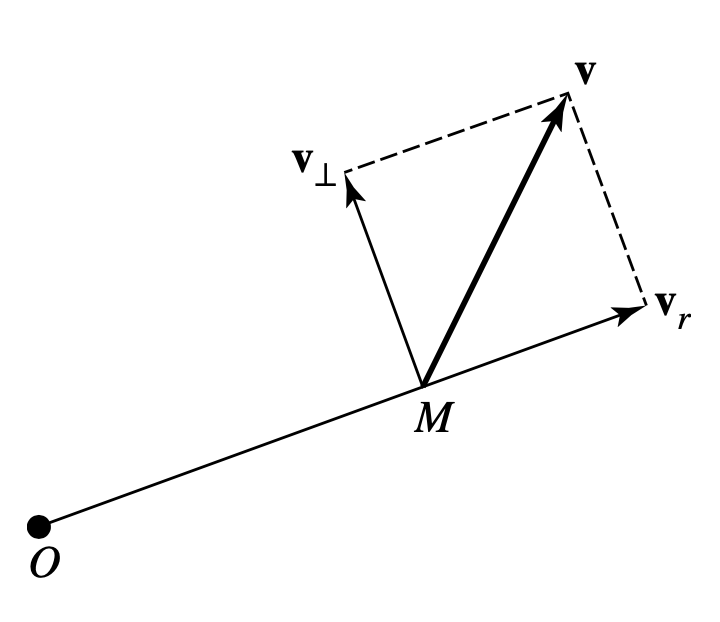
\includegraphics[scale=0.6]{fig/fig1-A-cohen.png}
		\caption{Radial component $\vb{v}_r$ and tangential component $\vb{v}_\perp$ of a particle's velocity.}
		\label{fig:1-a-cohen}
	\end{center}	
\end{figure}

Now let us consider Fig. \ref{fig:1-a-cohen} the position (denoted by $\vb{OM}=\vb{r}$) and velocity $\vb{v}$ of the particle at the instant $t$. Thw two vectors $\vb{r}$ and $\vb{v}$ lie in the plane of the trajectory and the velocity $\vb{v}$ can be decomposed into the radial component $\vb{v}_r$ (along the axis defined by $\vb{r}$) and the tangential component $\vb{v}_\perp$ (along the axis perpendicular to $\vb{r}$). The radual velocity, the algebraic value of $\vb{v}_r$, is the time derivative of the distance of the particle from the point $O$:
\begin{equation}\label{A-4}
	v_r=\dv{r}{t}
\end{equation}
The tangential velociry can be expressed in term of $r$ and the angular momentum $\vb{\mathcal{L}}$, since:
\begin{equation}\label{A-5}
	|\vb{r}\times\vb{v}|=r|\vb{v}_\perp|
\end{equation}
so that the modulus of the angular momentum $\vb{\mathcal{L}}$ is equal to:
\begin{equation}\label{A-6}
	|\vb{\mathcal{L}}|=|\vb{r}\times\mu\vb{v}|=\mu r|\vb{v}_\perp|
\end{equation}
The total energy of the particle:
\begin{equation}\label{A-7}
	E=\frac{1}{2}\mu\vb{v}^2+V(r)=\frac{1}{2}\mu \vb{v}_r^2+\frac{1}{2}\mu \vb{v}_\perp^2+V(r)
\end{equation}
can be written:
\begin{equation}\label{A-8}
	E=\frac{1}{2}\mu\vb{v}_r^2+\frac{\vb{\mathcal{L}}^2}{2\mu r^2}+V(r)
\end{equation}
The classical Hamiltonian if the system is then:
\begin{equation}\label{A-9}
	\mathcal{H}=\frac{p_r^2}{2\mu}+\frac{\vb{\mathcal{L}}^2}{2\mu r^2} + V(r)
\end{equation}
where:
\begin{equation}\label{A-10}
	p_r=\mu\dv{r}{t}
\end{equation}
is the conjugate momentum of $r$,  and $\vb{\mathcal{L}}^2$ must be expressed in terms of the variables $r, \theta, \varphi$ and their conjugate momenta $p_r,p_\theta,p_\varphi$. One finds:
\begin{equation}\label{A-11}
	\vb{\mathcal{L}}^2=p_\theta ^2 +\frac{1}{\sin^2\theta}p_\varphi^2
\end{equation}
In expression (\ref{A-9}), the kinetic energy is broken into two terms: the radial kinetic energy and the kinetic energy of rotation about $O$ . The reason is that, since $V(r)$ is independent of $\theta$ and $\varphi$ in this case, the angular variables and their conjugate momenta appear only in the $\vb{\mathcal{L}}^2$ term. In fact, if we are interested in the evolution of $r$, we can use the fact that $\vb{\mathcal{L}}$ is a constant of the motion, and replace $\vb{\mathcal{L}}^2$ by a constant in expression (\ref{A-9}). The Hamiltonian $\mathcal{H}$  then appears as a function only of the radial variables $r$ and $p_r$ ( $\vb{\mathcal{L}}^2$ plays the role of a parameter), and the result is a differential equation involving only one variable, $r$:
\begin{equation}\label{A-12a}
	\dv{p_r}{t}=\mu\dv[2]{r}{t}=-\pdv{\mathcal{H}}{r}
\end{equation}
that is:
\begin{equation}\label{A-12b}
	\mu\pdv[2]{r}{t}=\frac{\vb{\mathcal{L}}^2}{\mu r^2}-\dv{V}{r}
\end{equation}
It is just as if we had a one-dimensional problem (with $r$ varyng only between $0$ and $+\infty$), with a particle of mass $\mu$ subjected to the "efective potential":
\begin{equation}\label{A-13}
	V_{eff}(r)=V(r)+\frac{\vb{\mathcal{L}}^2}{2\mu r^2}
\end{equation}
We shall see that the situation is analogous in quantum mechanics.


\subsubsection{The quantum mechanical Hamiltonian}
In quantum mechanics, we want to solve the eigenvalue equation of the Hamiltonian $\mathcal{H}$, the observable associated with the total energy. This equation is written, in the $\{\ket{\vb{r}}\}$ representation:
\begin{equation}\label{A-14}
	\left[-\frac{\hbar^2}{2\mu}\Delta +V(r)\right]\varphi(\vb{r}) = E\varphi(\vb{r})
\end{equation}
Since the potential $V$ depends only on the distance  $r $of the particle from the origin, spherical coordinates are best adapted to the problem. We therefore express the Laplacian $\Delta$ in spherical coordinates \footnote{Expression (\ref{A-15}) gives the Laplacian only for non-zero $r$. This is because of the privileged position of the origin in spherical coordinates; it can be seen, moreover, that expression (\ref{A-15}) is not defined for $r=0$.}
\begin{equation}\label{A-15}
	\Delta = \frac{1}{r}\pdv[2]{r}r+\frac{1}{r^2}\left(\pdv[2]{\theta} +\frac{1}{\tan\theta}\pdv{\theta}+\frac{1}{\sin^2\theta}\pdv[2]{\varphi}\right)
\end{equation}
and look for eigenfucntions $\varphi(\vb{r})$ that are functions of the variables $r,\theta,\varphi$.

If we compare expression (\ref{A-15}) with the one for the operator $\vb{\mathcal{L}}^2$, wee see that the quantum mechanical Hamiltonian $\mathcal{H}$ can be put in a form completely analogous to (\ref{A-9}):
\begin{equation}\label{A-16}
	\boxed{H=-\frac{\hbar^2}{2\mu}\frac{1}{r}\pdv[2]{r}+\frac{1}{2\mu r^2}\vb{L}^2+V(r)}
\end{equation}
The angular dependence of the Hamiltonian is contained entirely in the $\vb{L}^2$ term, which is an operator here. We could, in fact, perfect the analogy by defining an operator $P_r$, which would allow us to write the first term of (\ref{A-16}) like the one in (\ref{A-9}).

We shall now show how one can solve the eigenvalue equation:
\begin{equation}\label{A-17}
	\left[-\frac{\hbar^2}{2\mu}\frac{1}{r}\pdv[2]{r}+\frac{1}{2\mu r^2}\vb{L}^2+V(r)\right]\varphi(r,\theta,\varphi)=E\varphi(r,\theta,\varphi)
\end{equation}

\subsection{Separation of variables}
\subsubsection{Angular dependence of the eigenfunctions}
We know that the three components of the angular momentum operator $\vb{L}$ act only on the angular variables $\theta$ and $\varphi$ ; consequently, they commute with all operators acting only on the $r$-dependence. In addition, they commute with $\vb{L}^2$. Therefore, according to expression (\ref{A-16}) for the Hamiltonian, \textit{the three components of L are constants of the motion\footnote{(\ref{A-18}) express the fact that $H$ is a scalar operator with respect to rotations about the point $O$. This is true because the potential energy is invariant under rotations about $O$.}} in the quantum mechanical sense:
\begin{equation}\label{A-18}
	[H,\vb{L}]=\vb{0}
\end{equation}

Obviously, $H$ also commutes with $\vb{L}^2$.

Although we have at our disposition four constants of the motion ($L_x,L_y,L_z$ and $\vb{L}^2$), we cannot use all four of them to solve equation (\ref{A-17}) because they do not commute with each other; we shall use only $\vb{L}^2$ and $L_z$. Since the three observables $H$, $\vb{L}^2$ and $L_z$ commute, we can find a basis of the state space $\mathcal{E}_r$ of the particle composed of eigenfunctions common to these three observables. We can, therefore,  require the functions $\varphi(r,\theta,\varphi)$, solutions of equation (\ref{A-17}), to be eigenfunctions of $\vb{L}^2$ and $L_z$  as well. We must then solve the system of differential equations:
\begin{align}
	\label{A-19a}H\varphi(\vb{r})&=E\varphi(\vb{r})\\
	\label{A-19b}\vb{L}^2\varphi(\vb{r})&=l(l+1)\hbar^2\varphi(\vb{r})\\
	L_z\varphi(\vb{r})&=m\hbar \varphi(\vb{r}) \label{A-19c}
\end{align}
But we already know the general form of the common eigenfunctions of $\vb{L}^2$ and $L_z$: the solutions $\varphi(\vb{r})$ of equations (\ref{A-19a}), (\ref{A-19b}), (\ref{A-19c}) corresponding to fixed values $l$ of and $m$ , are necessarily products of a function of $r$ alone and the spherical harmonic $Y_l^m(\theta,\varphi)$:
\begin{equation}\label{A-20}
	\varphi(\vb{r})=R(r)Y_l^m(\theta,\varphi)
\end{equation}
Whatever the radial function $R(r)$, $\varphi(\vb{r})$ is a solution of equations (\ref{A-19b}) and (\ref{A-19c}). The only problem which remains to be solved is therefore how to determine $R(r)$ such that $\varphi(\vb{r})$ is also an eigenfunction of $H$ [equation (\ref{A-19a})].

\subsubsection{The radial equation}
We shall now substitute expressions (\ref{A-16}) and (\ref{A-20}) into (\ref{A-19a}). Since $\varphi(\vb{r})$ is an eigenfunction of $\vb{L}^2$ with the eigenvalue $l(l+1)\hbar^2$, we see that $Y_l^m(\theta,\varphi)$ is a common factor on both sides. After simplifyng, we obtain the radial equation:
\begin{equation}\label{A-21}
	\left[-\frac{\hbar^2}{2\mu}\frac{1}{r}\dv[2]{r}r+\frac{l(l+1)\hbar^2}{2\mu r^2}+V(r)\right]R(r)=ER(r)
\end{equation}
Actually, a solution of (\ref{A-21}), substituted into (\ref{A-20}), does not necessarily yield a solution of the eigenvalue equation (\ref{A-14}) of the Hamiltonian. As we have already pointed out, expression (\ref{A-15}) for the Laplacian is not necessarily valid at $r=0$. We must therefore make sure that the behavior of the solutions $R(r$) of (\ref{A-21}) at the origin is sufficiently regular for (\ref{A-20}) to be in fact a solution of (\ref{A-14}).

Instead of solving the partial differential equation (\ref{A-17}) involving the three variables $r,\theta\varphi$ we must now solve a differential equation involving only the variable $r$, but dependent on a parameter $l$: we are looking for eigenvalues and eigenfunctions of an operator $H_l$ which is different for each value of $l$.

In other words, we consider separately, in the state space $\mathcal{E}_r$, the subspaces $\mathcal{E}(l,m)$ corresponding to fixed values of $l$ and $m$ , studying the eigenvalue equation of $H$ in each of these subspaces (which is possible because $H$ commutes with $\vb{L}^2$ and $L_z$). The equation to be solved depends on $l$ , but not on $m$ ; it is therefore the same in the $(2l+1)$ subspaces $\mathcal{E}(l,m)$ associated with a given value of $l$. We shall denote by $_{k,l}$ the eigenvalues of $H_l$ , that is, the eigenvalues of the Hamiltonian $H$ inside a given subspace $\mathcal{E}(l,m)$. The index $k$, which can be discrete or continuous, represents the various eigenvalues associated with the same value of $l$. As for the eigenfunctions of $H_l$, we shall label them with the same two indices as the eigenvalues: $R_{k,l}(r)$. It is not obvious that this is sufficient: several radial functions might exist and be eigenfunctions of the same operator $H_l$ with the same eigenvalue $E_{k,l}$; we shall see that this is not the case and that, consequently, the two indices $k $and $l$ are sufficient to characterize the different radial functions. We shall therefore rewrite equation (\ref{A-21}) in the form:
\begin{equation}\label{A-22}
	\left[-\frac{\hbar^2}{2\mu}\frac{1}{r}\dv[2]{r}+\frac{l(l+1)\hbar^2}{2\mu r^2}+V(r)\right]R_{k,l}(r)=E_{k,l}R_{k,l}(r)
\end{equation}
We can simplify the differential operator to be studied by a change in functions.

We set:
\begin{equation}\label{A-23}
	R_{k,l}(r)=\frac{1}{r}u_{k,l}(r)
\end{equation}
Multiplying both sides of (\ref{A-22}) by $r$, we obtain for $u_{k,l}(r)$ the following differential equation:
\begin{equation}\label{A-24}
	\boxed{\left[-\frac{\hbar^2}{2\mu}\dv[2]{r}+\frac{l(l+1)\hbar^2}{2\mu r^2}+V(r)\right]u_{k,l}(r)=E_{k,l}(r)u_{k,l}(r)}
\end{equation}
This equation is analogous to the one we would have to solve if, in a \textit{one-dimensional} problem, a particle of mass $\mu$ were moving in an \textit{effective potential} $V_{eff}(r)$: 
\begin{equation}\label{A-25}
	V_{eff}(r)=V(r)+\frac{l(l+1)\hbar^2}{2\mu r^2}
\end{equation}
Nevertheless, we must not lose sight of the fact that the variable $r$ can take on only \textit{non-negative} real values. The term $l(l+1)\hbar^2/2\mu r^2$ which is added to the potentual $V(r)$ is always positive or zero; the corresponding force (equal to minus the gradient of this term) always tend to repel the particle from the force center $O$; this is whay this term is called the \textit{centrifugal potential} (or centrifugal barrier).

\subsubsection{Behavior of the solutions of the radial equation at the origin}\label{sec:A-2-c}
We have already pointed out that it is necessary to examine the behavior of the solutions $R(r)$ of the radial equation (\ref{A-21}) at the origin in order to know if they are really solutions of (\ref{A-14}).

We shall assume that when $r$ approaches zero, the potential $V(r)$ remains finite, or at least approaches infinity less rapidly than $1/r$ (this hypothesis is true in most cases encountered in physics and, in particular, in the case of the Coulomb potential. We shall consider a solution of (\ref{A-22}) and assume that it behaves at the origin like $r^s$:
\begin{equation}\label{A-26}
	R_{k,l}(r)\thicksim Cr^s\quad \mbox{,as } r\to 0
\end{equation}
Substituting (\ref{A-26}) into (\ref{A-22}), and setting the coefficient of the dominant term equal to zero, we obtain the equation:
\begin{equation}
	-s(s+1) + l(l+1)=0
\end{equation}
and, consequently:

\begin{equation}\label{A-28}
	\left \{
		\begin{array}{ccc}
			\mbox{either} & s=l\\
			\mbox{or}  & s=-(l+1)
		\end{array}
	\right.
\end{equation}

For a given value of $E_{k,l}$, there are therefore two linearly independent solutions of the second-order equation (\ref{A-22}), behaving at the origin like $r^l$ and $1/R^{l+1}$, respectively. But those which behave like $1/r^{l+1}$ must be rejected, since it can be shown\footnote{This is because the Laplacian of $\frac{1}{r^{l+1}}Y_l^m(\theta,\varphi)$ involves the $l$th derivatives of $\delta(\vb{r})$.} that $\frac{1}{r^{l+1}}Y_l^m(\theta,\varphi)$ is not a solution of the eigenvalue equation (\ref{A-14}) for $r=0$. From this, we see that acceptable solution of (\ref{A-24}) go to zero at the origin for all $l$, since:
\begin{equation}\label{A-29}
	u_{k,l}(r)\thicksim Cr^{l+1}\quad  \mbox{,as } r\to 0
\end{equation}
Consequantly, to (\ref{A-24}) must be added the condition:
\begin{equation}\label{A-30}
	\boxed{u_{k,l}(0)=0}
\end{equation}

\subsection{Statioanary states of a particle in a central potential}
\subsubsection{Quantum numbers}
We can summarize the results as follows: the fact that the potential $V(r)$ is independent of $\theta$ and $\varphi$ makes it possible:
\begin{enumerate}
	\item to require the eigenfunctions of $H$ to be \textit{simultaneous eigenfunctions} of $\vb{L}^2$ \textit{and} $L_z$, \textit{which determines their angular dependence}:
		\begin{equation}\label{A-31}
	\varphi_{k,l,m}(\vb{r})=R_{k,l}(r)Y_l^m(\theta,\varphi)=\frac{1}{r}u_{k,l}(r)Y_l^m(\theta,\varphi)
\end{equation}
\item \textit{to replace the eigenvalue equation of} $H$, an equation involving partial derivatives with respect to $r,\theta,\varphi$ by a \textit{differential equation involving only the variable} $r$ and depending on a parameter $l$ [(\ref{A-24})], with condition (\ref{A-30}) imposed.
\end{enumerate}

In principle, the functions $\varphi_{k,l,m}(r,\theta,\varphi)$ must be squre-integrable, that is, normalizable:
\begin{equation}\label{A-32}
	\int |\varphi_{k,l,m}(r,\theta,\varphi)|^2r^2\dd r\dd \Omega = 1
\end{equation}
Their form (\ref{A-31}) allows us to separate radial and angular integrations:
\begin{equation}\label{A-33}
	\int |\varphi_{k,l,m}(r,\theta,\varphi)|^2r^2\dd r\dd \Omega =\int_0^\infty r^2\dd r R_{k,l}(r)|^2\int \dd\Omega |Y_l^m(\theta,\varphi)|^2
\end{equation}
But the spherical harmonics $Y_l^m(\theta,\varphi)$ are normalized with respect to $\theta$ and $\varphi$; condition (\ref{A-32}) therefore reduces to:
\begin{equation}\label{A-34}
	\int_0^\infty r^2\dd r |R_{k,l}(r)|^2=\int_0^\infty \dd r |u_{k,l}(r)|^2=1
\end{equation}
Actually, we know that it is often convenient to accept eigenfunctions of the Hamil- tonian that are not square-integrable. If the spectrum of $H$ has a continuous part, we shall require only that the corresponding eigenfunctions be orthonormalized in the ex- tended sense, that is, that they satisfy a condition of the form:
\begin{equation}\label{A-35}
	\int_0^\infty r^2\dd r R_{k,l}^*(r)R_{k,l}(r)=\int_0^\infty \dd r u_{k,l}^*(r)u_{k,l}(r)=\delta(k'-k)
\end{equation}
where $k$ is a continuous index.
In (\ref{A-34}) and (\ref{A-35}), the integrals converge at their lower limit, $r=0$ [condition (\ref{A-30})]. This is physically satisfying since the probability of finding the particle in any volume of finite dimensions is then always finite. It is therefore only because of the behavior of the wave functions for $r\to \infty$ that, in the case of a continuous spectrum, the normalization integrals (\ref{A-35}) diverge if $k=k'$.

Finally, the eigenfunctions of the Hamiltonian $H$ of a particle placed in a central potential $V(r)$ depend on at least three indices [formula (\ref{A-31})]: $\varphi_{k,l,m}(r,\theta,\varphi)=R_{k,l}(r)Y_l^m(\theta,\varphi)$ is a somultaneous eigenfunction of $H, \vb{L}^2$ and $L_z$ with the respective eigenvalues $E_{k,l}, l(l+1)\hbar^2$ and $m\hbar$. $k$ is called the \textit{radial} quantum number; $l$, the \textit{azimuthal} quantum number; and $m$ the \textit{magnetic} quantum number. The radial part $R_{k,l}(r)=\frac{1}{r}u_{k,l}(r)$ of the eigenfunction and the eigenvalue $E_{k,l}$ of $H$ are independent of the magnetic quantum number and are given by the radial equation (\ref{A-24}). The angular part of the eigenfunction depends only on $l$ and $m$ and not on $k$; it does not depend on the form of the potentual $V(r)$.

\subsubsection{Degeneracy of the energy levels}

\section{Potion of the center of mass and relative motion for a system fo two interacting particles}

\subsection{Motion od the center of masss and relative motion in classical mechanics}

\subsection{Separation of variables in quantum mechanics}
\subsubsection{Eigenvalues and eigenfunctions of the Hamiltonian}

\section{The hydrogen atom}
\subsection{Introduction}
The hydrogen atom consists of a proton, of mass:
\begin{equation}\label{C-1}
	m_p\approx 1.7\times 10^{-27} \mbox{ kg}
\end{equation}
and charge:
\begin{equation}\label{C-2}
	q\approx 1.6\times 10^{-19} \mbox{ Coulomb}
\end{equation}
and of and electron, of mass:
\begin{equation}\label{C-3}
	m_e\approx 0.91\times 10^{-30}\mbox kg
\end{equation}
and a charge $-q$. The interaction between these two particles is essentially electrostatic. The corresponding potential energy is:
\begin{equation}\label{C-4}
	V(r)\approx -\frac{q^2}{4\pi\epsilon_0}\frac{1}{r}=-\frac{e^2}{r}
\end{equation}
where $r$ denotes the distance between the two particles, and:
\begin{equation}\label{C-5}
	\frac{q^2}{4\pi\epsilon_0}=e^2
\end{equation}
We confine ourselves to the study of this system in the center of mass frame. The classical Hamiltonian that describes the relative motion of the two particles is then:
\begin{equation}\label{C-6}
	\mathcal{H}(\vb{r},\vb{p})=\frac{\vb{p}^2}{2\mu}-\frac{e^2}{r}
\end{equation}
Since $m_p \gg m_e$ [formulas (\ref{C-1}) and (\ref{C-3})], the reduced mass $\mu$ of the system is very close to $m_e$:
\begin{equation}\label{C-7}
	\mu=\frac{m_em_p}{m_e+m_p}\approx m_e\left(1-\frac{m_e}{m_p}\right)
\end{equation}
(the correction term $m_e/m_p$ is on the order of $1/1800$).  This means that the center of mass of the system is practically at the position of the proton, and that the relative particle can be identified, to a very good approximation, with the electron. This is why we shall adopt the slightly inaccurate convention of calling the relative particle the electron and the center of mass the proton.

\subsection{The Bohr model}
We shall briefly review the results of the Bohr model, which relate to the hydrogen atom. This model, which is based on the concept of a trajectory, is incompatible with the ideas of quantum mechanics. However, it allows us to introduce, in a very simple way, fundamental quantities such as the ionization energy $E_I$ of the hydrogen atom and a parameter which characterizes atomic dimensions (the Bohr radius $a_0$). In addition, it so happens that the energies $E_n$ given by the Bohr theory are the same as the eigenvalues of the Hamiltonian we shall calculate in \ref{sec:C-3}. Finally, quantum mechanical theory is in agreement with some of the intuitive images of the Bohr model.

This semi-classical model is based on the hypotesis that the electron describes a \textit{circular orbit} of radius $r$ about the proton, obeying the following equations:
\begin{align}
	\label{C-8}E&=\frac{1}{2}\mu v^2-\frac{e^2}{r}\\
	\label{C-9}\frac{\mu v^2}{r}&=\frac{e^2}{r^2}\\
	\mu  v r&=n\hbar\quad ; \quad \mbox{$n$ a positive number}\label{C-10}
\end{align}
The first two equations are classical ones. (\ref{C-8}) expresses the fact that the total energy $E$ of the electron is the sum of its kinetic energy $\mu v^2/2$  and its potential energy $-e^2/r$ . (\ref{C-9}) is none other than the fundamental equation of Newtonian dynamics ($e^2/r^2$ is the Coulomb force exerted on the electron, and $v^2/r$ is the acceleration of its uniform circular motion). The third equation expresses the quantization condition, introduced empirically by Bohr in order to explain the existence of discrete energy levels: he postulated that only circular orbits satisfying this condition are possible trajectories for the electron. The different orbits, as well as the corresponding values of the various physical quantities, are labeled by the integer $n$ associated with them.

A very simple algebraic calculation then yields the expressions for $E_n,r_n$ and $v_n$:
\begin{align}
	\label{C-11a}E_n&=-\frac{1}{n^2}E_I\\
	\label{C-11b}r_n&=n^2a_0\\
	v_n&=\frac{1}{n}v_0\label{C-11c}
\end{align}
with 
\begin{align}
	\label{C-12a}E_I&=\frac{\mu e^4}{2\hbar^2}\\
	\label{C-12b}a_0&=\frac{\hbar^2}{\mu e^2}\\
	v_0&=\frac{e^2}{\hbar}\label{C-12c}
\end{align}
When this model was proposed by Bohr, it marked an important step towards the understanding of atomic phenomena, since it yielded the correct values for the energy level of the hydrogen atom. These values indeed follow the $1/n^2$ (the Balmer formula) law indicated by expression (\ref{C-11a}). Moreover, the experimentally measured \textit{ionization energy} (the energy which must be supplied to the hydrogen atom in its ground state in order to remove the electron) is equal to the numerical value of $E_I$:
\begin{equation}\label{C-13}
	E_I\approx 13.6 \mbox{ eV }
\end{equation}
Finally, the \textit{Bohr radius} $a_0$ indeed characterized atomix¡c dimensions:
\begin{equation}\label{C-14}
	a_0\approx 0.52  \,\si{\angstrom}
\end{equation}

\subsection{Quantum mechanical theory of the hydrogen atom}\label{sec:C-3}
We shall now take up the question of the determination of the eigenvalues and eigenfunctions of the Hamiltonian $H$ describing the relative motion of the proton and
the electron in the center of mass frame [formula (\ref{C-6})]. In the $\{\ket{\vb{r}}\}$ representation, the eigenvalue equation of the Hamiltonian $H$ is written:
\begin{equation}\label{C-15}
	\left[-\frac{\hbar^2}{2\mu}\Delta -\frac{e^2}{r}\right]\varphi(\vb{r})=E\varphi(\vb{r})
\end{equation}
Since the potential $-e^2/r$ is central, we can apply the results of \ref{sec:A}: the eigenfunctions $\varphi(\vb{r})$ are of the form:
\begin{equation}\label{C-16}
	\varphi_{k,l,m}(\vb{r})=\frac{1}{r}u_{k,l}(r)Y_l^m(\theta,\varphi)
\end{equation}
$u_{k,l}(r)$ is given by the radial equation, (\ref{A-24}), that is:
\begin{equation}\label{C-17}
	\left[-\frac{\hbar^2}{2\mu}\dv[2]{r}+\frac{l(l+1)\hbar^2}{2\mu r^2}-\frac{e^2}{r}\right]u_{k,l}(r)=E_{k,l}(r)u_{k,l}(r)
\end{equation}
We add to this equation condition (\ref{A-30}):
\begin{equation}\label{C-18}
	u_{k,l}(0)=0
\end{equation}

\subsubsection{Change of variables}
To simplify the reasoning, we shall choose $a_0$ and [formulas (\ref{C-12a}), (\ref{C-12b}) and (\ref{C-12c})] as the units of length and energy. That is, we shall introduce the dimensionless quantities:
\begin{equation}\label{C-19}
	\rho = r/a_0
\end{equation}
\begin{equation}\label{C-20}
	\lambda_{k,l}=\sqrt{-E_{k,l}/E_I}
\end{equation}
(the quantity under the radical sign is positive, since we are looking for the bound states).

With expressions (\ref{C-12a}) and (\ref{C-12b}) for $E_I $and $a_0$ taken into account, the radial equation (\ref{C-17}) becomes simply:
\begin{equation}\label{C-21}
	\left[\dv[2]{\rho}-\frac{l(l+1)}{\rho^2}+\frac{2}{\rho}\right]u_{k,l}(\rho)=0
\end{equation}

\subsubsection{Solving the radial equation}
In order to solve (\ref{C-21}), we shall expanding $u_{k,l}(\rho)$ in a power series.

\begin{itemize}
	\item Asymptotic behavior

		Let us determine the asymptotic behavior of $u_{k,l}(\rho)$ qualitatively. When $\rho$ approaches infinity, the terms in $1/\rho$ and $1/\rho^2$ become negligible compared to the constant term $\lambda_{k,l}^2$, so that (\ref{C-21}) practically reduces to:
		\begin{equation}\label{C-22}
			\left[\dv[2]{\rho}-\lambda_{k,l}^2\right]u_{k,l}(\rho)=0
\end{equation}
whose solutions are $e^{\pm\rho\lambda_{k,l}}$. This argument is not rigorous, since we have completely neglected the terms in $1/\rho$ and $1/\rho^2$; actually, it can be shown that $u_{k,l}(\rho)$ is equal to $E^{\pm\rho\lambda_{k,l}}$ multiplied by a power of $\rho$.

We shall later be led by physical considerations to require the function $u_{k,l}(\rho)$ to be bounded at infinity, and hence to reject the solutions of (\ref{C-21}) whose asymptotic behavior is governed by $e^{+\rho\lambda_{kl}}$ . This is why we perform the change of function:
\begin{equation}\label{C-23}
	u_{k,l}(\rho)=e^{-\rho\lambda_{k,l}}y{k,l}(\rho)
\end{equation}
Although this change of function singles out $e^{-\rho\lambda_{k,l}}$ , it clearly does not eliminate solutions in $e^{+\rho\lambda_{k,l}}$ , which must be identified and then rejected at the end of the calculation. The differential equation that $y_{k,l}(\rho)$ must satisfy can easily be derived from (\ref{C-21}):
\begin{equation}\label{C-24}
	\left\{\dv[2]{\rho}-2\lambda_{k,l}\dv{\rho}+\left[\frac{2}{\rho}-\frac{l(l+1)}{\rho^2}\right]\right\}y_{k,l}(\rho)=0
\end{equation}
Condition (\ref{C-18}) must be associated with this equation, that is:
\begin{equation}\label{C-25}
	y_{k,l}(\rho)=0
\end{equation}
\item Solutions in the form of power series

	Consider de expansion of $y_{k,l}(\rho)$ in a powers of $\rho$:
	\begin{equation}\label{C-26}
	y_{k,l}(\rho)=\rho^s\sum_{q=0}^\infty c_q\rho^q
\end{equation}
By definition, $c_0$ is the first non-zero coefficient of this expansion:
\begin{equation}\label{C-27}
	c_0\neq 0
\end{equation}
Condition (\ref{C-25}) implies that $s$ is stricly positive.

We calculate $\dv{\rho}y_{k,l}(\rho)$ and $\dv[2]{\rho}y_{k,l}(\rho)$ from (\ref{C-26}):
\begin{align}
	\label{C-28a}\dv{\rho}&=\sum_{q_0}^\infty (q+s)c_q\rho^{q+s-1}\\
	\dv[2]{\rho}y_{k,l}(\rho)&=\sum_{q=0}^\infty (q+s)(q+s-1)c_1\rho^{q+s-2}\label{C-28b}
\end{align}
To obtain the left-hand side of (\ref{C-24}), we multiply expressions (\ref{C-26}), (\ref{C-28a}) and (\ref{C-28b}) respectively by the factors $\left[\frac{2}{\rho}-\frac{-(l+1)}{\rho^2}\right]$, $-2\lambda_{k,l}$ and $1$. According to (\ref{C-24}), the series to determined must ve identically zero, that is, all ist coefficients must be zero.

The lowest term is in $\rho^{s-2}$. Taking its coefficient as zero, we obtain:
\begin{equation}\label{C-29}
	[-(l+1)+s(s-1)]c_0=0
\end{equation}
If we take (\ref{C-27}) into account, we see that $s$ can take on one of two values:
\begin{equation}\label{C-30}
	\left \{
		\begin{array}{cc}
			s&=l+1\\
			s&=-l
		\end{array}
	\right.
\end{equation}
(in agreement with the general result of \ref{sec:A-2-c}). We have seen that only (\ref{A-30a}) gives a behavior at the origin that can lead to an acceptable solution [condition (\ref{C-25})]. Setting the coefficient of the general term in $\rho^{q+s-2}$ equal to zero, we obtain (with $s=l+1$) the following recurrence relation:
\begin{equation}\label{C-31}
	q(q+2l+1)c_q=2[(q+l)\lambda_{k,l}-1]c_{q-1}
\end{equation}
If we fix $c_0$, this relation enables us to calculate $c_1$, then $c_2$m and thus by recurrence all the coefficients $c_q$. Since $c_1/c_{q-1}$ approaches zero when $q\to 0$, the corresponding series is convergent for all $\rho$. Thus we have determined, for any value of $\lambda_{k,l}$, the solution of (\ref{C-24}) that satisfies condition (\ref{C-25}).
\end{itemize}

\subsubsection{Energy quantization. Radial functions}
We are now going to require the preceding solution to have a physically acceptable asymptotic behavior. This will involve quantization of the possible values of $\lambda_{k,l}$.

If the term in brackets on the right-hand side of (\ref{C-31}) does not go to zero for any integer $q$, expansion (\ref{C-26}) is a true infinite series, for which:
\begin{equation}\label{C-32}
	\frac{c_1}{c_{q-1}}\thicksim \frac{2\lambda_{k,l}}{q}\quad \mbox{,as $q\to\infty$}
\end{equation}
Now, the power series expansion of the function $e^{2\lambda_{k,l}}$ is written:

\begin{equation}\label{C-33}
	\left \{
		\begin{array}{cc}
			e^{2\rho\lambda_{k,l}}&=\sum_{q=0}^\infty d_q\rho^q\\
			d_q&=\frac{(2\lambda_{k,l})^q}{q!}
		\end{array}
	\right.
\end{equation}
which implies:
\begin{equation}\label{C-34}
	\frac{d_1}{d_{q-1}}=\frac{2\lambda_{k,l}}{q}
\end{equation}
If we compare (\ref{C-32}) and (\ref{C-34}), we see that, for large values of $\rho$ , the series being considered behaves like $e^{2\rho\lambda_{k,l}}$. The corresponding function $u_{k,l}$ [formula (\ref{C-23})] is then proportional to $e^{+\rho\lambda_{k,l}}$ , which is not physically acceptable.

Consequently, we must reject all cases in which expansion (\ref{C-26}) is an infinite series. The only possible values of $\lambda_{k,l}$ are those for which (\ref{C-26}) has only a finite number of terms, that is, those for which $y_{k,l} $reduces to a polynomial. The corresponding function $u_{k,l}$ is then physically acceptable, since its asymptotic behavior is dominated by $e^{-\rho\lambda_{k,l}}$ . Therefore, all we need is an integer $k$ such that the term in brackets of the right-hand side of (\ref{C-31}) goes to zero for $q=k$: the corresponding coefficient $c_k$ is then zero, as are all those of higher order, since the fact that $c_k$ is zero means that $c_{k+1}$ is as well, and so on. For fixed $l$, we label the corresponding values of $\lambda_{k,l}$ by this integer $k$ (note that $k$ is greater than or equal to $1$, since $c_0$ never goes to zero). We then have, according to (\ref{C-31}):
\begin{equation}\label{C-35}
	\lambda_{k,l}=\frac{1}{k+l}
\end{equation}
For a given $l$, the only negative energies possible are therefore [formula (\ref{C-20})]:
\begin{equation}\label{C-36}
	E_{k,l}=\frac{-E_I}{(k+l)^2};\qquad k=1,2,3,...
\end{equation}
We shall discuss this result in \ref{sec:C-4}

$y_{k,l}$ is therefore a polynomial, whose term of lowest order is in $\rho^{l+1}$ and whose term of highest order is in $\rho^{k+l}$ . Its various coefficients can be calculated in terms of $c_0$ by solving recurrence relation (\ref{C-31}), which can be written, using (\ref{C-35}):
\begin{equation}\label{C-37}
	c_q=-\frac{2(k-q)}{q(q+2l+1)(k+l)}c_{q-1}
\end{equation}
It is easy to show that:
\begin{equation}\label{C-38}
	c_q=(-1)^q\left(\frac{2}{k+l}\right)^q\frac{(k-1)!}{(k-q-1)!}\frac{(2l+1)!}{q!(q+2l+1)!}c_0
\end{equation}
$u_{k,l}$ is then given by formula (\ref{C-23}), and $c_0$ is determined (to within a phase factor) by normalization condition (\ref{A-34}) [we must first, of course, return to the variable $r$ by using (\ref{C-19})]. Finally, we obtain the true function $R_{k,l}(r)$ by dividing $u_{k,l}(r)$ by $r$. The following three examples give an idea of the form of these radial functions:
\begin{align}
	\label{C-39a}R_{k=1,l=0}(r)&=2(a_0)^{-3/2}e^{-r/a_0}\\
	\label{C-39b}R_{k=2,l=0}(r)&=2(a_0)^{-3/2}\left(1-\frac{r}{2a_0}\right)e^{-r/2a_0}\\
	R_{k=1,l=1}(r)&=(2a_0)^{-3/2}\frac{1}{\sqrt{3}}\frac{r}{a_0}e^{-r/2a_0}\label{C_39c}
\end{align}

\subsection{Discussion of the results}\label{sec:C-4}
\subsubsection{Order if magnitude of atomic parameters}
Formulas (\ref{C-36}) and (\ref{C-39}) show that, for the hydrogen atom, the ionization energy , defined by (\ref{C-12a}), and the Bohr radius, given by (\ref{C-12b}), play an important role. These quantities give an order of magnitude of the energies and spatial extensions of the wave functions associated with the bound states of the hydrogen atom.

Relations (\ref{C-12a}) and (\ref{C-12b}) can be written in the form:
\begin{align}
	\label{C-40a}E_I&=\frac{1}{2}\alpha^2\mu c^2\\
	a_0&=\frac{1}{\alpha}\lambdabar_c\label{C-40b}
\end{align}
where $\alpha$ is the \textit{fine structure constant}, a dimensionless constant which plays a very important role in physics:
\begin{equation}\label{C-41}
	\alpha = \frac{e^2}{\hbar c}=\frac{q^2}{4\pi\epsilon_0 \hbar c}\approx\frac{1}{137}
\end{equation}
and where $\lambdabar_c$ is defined by:
\begin{equation}\label{C-42}
	\lambdabar_c = \frac{\hbar}{\mu c}
\end{equation}
Sinse $\mu$ is almost the same as $m_e$, the rest mass of the electron, $\lambdabar_c$ is practically equal to the \textit{Compton wavelength} of the electron, which is given by:
\begin{equation}
	\frac{\hbar}{m_ec}\approx 3.8\times 10^{-3}\, \si{\angstrom}
\end{equation}
Relation (\ref{C-40b}) therefore indicates that $a_0$ is on the order of one hundred times the Compton wavelength of the electron. Relation (\ref{C-40a}) shows that the order of magnitude of the binding energy of the electron is between $10^{-4}\mu c^2$ and $10^{-5}\mu c^2$, where $\mu c^2$ is practically equal to the rest energy of the electron:
\begin{equation}\label{C-44}
	m_ec^2\approx 0.51\times 10^6\, \mbox{eV}
\end{equation}
It follows that:
\begin{equation}\label{C-45}
	E_I\ll m_ec^2
\end{equation}

\subsubsection{Energy levels}
\begin{itemize}
	\item \textit{Possible values of the quantum numbers; degeneracies}


		For fixed $l$, there exists an infinite number of possible energy values [formula (\ref{C-36})], corresponding to $k= 1, 2, 3$, ... Each of them is at least $(2 + 1)$-fold degenerate: this is an \textit{essential degeneracy} related to the fact that the radial equation depends only on the quantum number $l$ and not on $m$ (\ref{sec:A-3})). But, in addition, there exist \textit{accidental degeneracies}: equation (\ref{C-36}) indicates that two eigenvalues $E_{k,l}$ and $E_{k',l'}$ corresponding to different radial equations $(l'\neq l)$ are equal if $k+l=k'+l'$. 

		In the special case of the hydrigen atom, $E_{k,l}$ does not depend on $k$ and $l$ separately, but only on their sum. We set:
		\begin{equation}\label{C-46}
	n = k+l
\end{equation}
The various energy states are labeled by the integer $n$ (greater than or equal to $1$), and (\ref{C-36}) becomes:
\begin{equation}\label{C-47}
	E_n=-\frac{1}{n^2}E_I
\end{equation}
According to (\ref{C-46}), it is equivalent to specify $k$ and $l$ or $n$ and $l$ to determine the eigenfunctions. Following convention, from now on we shall use the quantum numbers $n$ and $l$. The energy is fixed by $n$, which is called the \textit{`principal quantum number}; a given value of $n$ characterizes what is called an \textit{electron shell}.

Since $k$ is necessarily an integer which is greater than or equal to $1$, there is only a finite number of values of $l$ associated with the same vale¡ue of $n$. According to (\ref{C-46}), if $n$ is fixed, one can have:
\begin{equation}\label{C-48}
	l=0,1,2,...,n-1
\end{equation}
The shell characterized by $n$ is said to contain $n$ \textit{sub-shells}, each one corresponding to one of the values $l$ of given in (\ref{C-48}). Finally, each sub-shell contains $(2l+1)$ distinct states, associated with the $(2l+1)$ possible values of $m$ for fixed $l$.

The total degeneracy of the energy level $E_n$ is therefore:
\begin{equation}\label{C-49}
	g_n=\sum_{l=0}^{n-1}(2l+1)=2\frac{(n-1)n}{2}+n=n^2
\end{equation}
We sall see that the existence of electron spin multiplies this number by $2$ (if we also take into account the proton spin, which is equal to that of the electron, we obtain another factor of $2$).

\item \textit{Spectroscopic notation}

For historical reasons (dating from the period, before the development of quantum mechanics, in which the study of spectra resulted in an empirical classification of the numerous lines observed), letters of the alphabet are associated with the various values of $l$. The correspondence is as follows:
\begin{align*}
	l&=0\leftrightarrow s\\
	l&=1\leftrightarrow p\\
	l&=2\leftrightarrow d\\
	l&=3\leftrightarrow f\\
	l&=4\leftrightarrow g\\
	\vdots & \vdots
	%\mbox{alphabetical order}
\end{align*}
Therefore, \textit{spectroscopic notation} labels a sub-shell by the corresponding number $n$ followed by the letter that characterizes the value of $l$. Thus, the ground level [which is non-degenerate, according to (\ref{C-49})], sometimes called the "$K$ shell", includes only the $1s$ sub-shell; the first excited level, or "$L$ shell", includes the $2s$ and $2p$ sub-shells; the second excited level ("$M$ shell") includes the $3s$ , $3p$ and $3d$ sub-shells, etc. (The capi- tal letters sometimes associated with the successive shells follow an alphabetical order, starting with the letter $K$.)
\end{itemize}

\subsubsection{Wave functions}\label{sec:C-4-c}
The wave functions associated with the eigenstates common to $\vb{L}^2$, $L_z$ and the Hamiltonian $H$ of the hydrogen atom are generally labeled, not by the three quantum numbers $k,l,m$ as we have done until now, but by $n$,$l$ and $m$ [passage from one set to the other simply involves use of relation (\ref{C-46})]. Since the operators $H, $$\vb{L}^2$ and $L_z$ constitute a C.S.C.O. (cf. \ref{A-3}), specification of the three integers $n,l$ and $m$ which is equivalent to that of the eigenvalues of $H$, $\vb{L}^2$ and $L_z$, unambiguously determines the corresponding eigenfunction $\varphi_{n,l,m}(\vb{r})$.

\begin{itemize}
	\item \textit{Angular dependence}

		As is the case for any central potential, the functions $\varphi_{n,l,m}(\vb{r})$ are products of a radial function and a spherical harmonic $Y_l^m(\theta,\varphi)$.To visualize their angular dependence on the axis characterized by the polar angles $\theta$ and $\varphi$, we can measure off a distance that is proporcional to $|\varphi_{n,l,m}(r,\theta,\varphi)|^2$ for any \textit{fixed} $r$, that is, proportional to $|Y_l^m(\theta,\varphi)|^2$. Thys, we obtain a surface of revolution about $Oz$ axis, since we know squently, $|Y_l^m(\theta,\varphi)|^2$ is independent of $\varphi$. We can therefore represent its cross-section by a plane containing $Oz$.

	\item \textit{Radial dependence}

		The radial functions $R_{n,l}(r)$, each of which characterizes a sub-sehll, can be calculated from the results of \ref{sec:C-3-c}, paying attention, however, to the change in notation introduced by formula (\ref{C-46}). 
		
		Finally, we can derive formula (\ref{C-11b}) for the successive Bohr radio. To do so, consider the various states for which $l=n$. We calculate the variation with of the probability density for each of the preceding levels in an infinitesimal solid angle $\dd \Omega$ about a fixed direction of polar angles $\theta$ and $\varphi$. In general, the position probability for the electron in the volume element $\dd^3 r=r^2\dd r\dd\Omega$ situated at the point $(r,\theta,\varphi)$ is given by:
\begin{align}\
	\nonumber \dd^3\mathcal{P}_{n,l,m}(r,\theta,\varphi)&=|\varphi_{n,l,.}(r,\theta,\varphi)|^2r^2\dd r\dd\Omega\\
																											 &=|R_{n,l}(r)|^2r^2\dd r\times |Y_l^m(\theta,\varphi)|^2\dd\Omega\label{C-52}
\end{align}
Here, we have fixed $\theta$, $\varphi$ and $\dd\Omega$. The probability of finding the electron between $r$ and $r+\dd r$ , inside the solid angle under consideration, is then proportional to $r^2|R_{n,l}(r)|^2\dd r$ . The corresponding density is therefore, to within a constant factor, $r^2|R_{n,l}(r)|^2$ (the factor $r^2$ arises from the expression for the volume element in spherical coordinates). We are interested in the case where $l=n-1$, that is, $k=n-l=1$; \ref{sec:C-3-c} then indicates
that the polynomial which enters into $R_{n,l}(r)$ contains only one term in $(r/a_0)^{n-1}$ desired probability density is therefore proportional to:
\begin{align}
	\nonumber f_n(r)&=\frac{r^2}{a_0^2}\left[\left(\frac{r}{a_0}\right)^{n-1}e^{r/na_0}\right]^2\\
									&=\left(\frac{r}{a_0}\right)^{2n}e^{-2r/na_0}\label{C-54}
\end{align}
This function has a maximum for:
\begin{equation}\label{C-54}
	r=r_n=n^2a_0
\end{equation}
which is the radius of the Bohr orbit corresponding to the energy $E_n$.


\end{itemize}




































\end{document}
